\documentclass{article}
\usepackage{geometry}
\geometry{
 a4paper,
 total={170mm,257mm},
 left=20mm,
 top=20mm,
 }
\usepackage[utf8]{inputenc}
\usepackage{kotex}
\usepackage{amsmath}
\usepackage{amssymb}
\usepackage{tikz}
\usetikzlibrary{shapes,arrows,positioning,calc}
\newcommand{\shah}[1]{\mathrm{III}\left(#1\right)}
\newcommand{\rect}[1]{\mathrm{rect}\left(#1\right)}
\newcommand{\sinc}[1]{\mathrm{sinc}\left(#1\right)}
\newcommand{\ft}[1]{\mathcal{F}\left\{#1\right\}}
\newcommand{\lt}[1]{\mathcal{L}\left\{#1\right\}}
\tikzset{
block/.style = {draw, fill=white, rectangle, minimum height=3em, minimum width=3em},
tmp/.style  = {coordinate}, 
sum/.style= {draw, fill=white, circle, node distance=1cm},
input/.style = {coordinate},
output/.style= {coordinate},
pinstyle/.style = {pin edge={to-,thin,black}
}
}
\title{Signals and Systems: Lecture Notes}
\author{서울대학교 전기$\cdot$정보공학부 430.306}
\begin{document}
\maketitle
\section{Lecture 2, 3}
\begin{itemize}

\item Signal: a function of independent variables

\item Harmonically related complex exponential:
Sets of periodic exponentials with common period $T$.\[\exp\left(j2\pi\left(\dfrac{kt}{T}\right)\right)(k\in\mathbb{Z})\]

\item Periodicity Properties of Discrete-Time Sinusoidal Signals:
\begin{enumerate}
\item Frequency uniquely defined in an interval with length 1. $[-1/2, 1/2)$

\item Periodicity: only if $f$ = rational number

\item $f_0$ = rational number, uniquely defined in the interval of definition
$N_{fund}$ = smallest positive integer which is a multiple of 1/$f_0$

$f_{fund}=1/N_{fund}$
\end{enumerate}
\item Definition of delta functions/unit step functions
\begin{itemize}
    \item $\delta(t)=\begin{cases}\infty(t=0)\\
    0(t\neq0)\end{cases}$, 
    $\displaystyle\int_{-\infty}^{\infty}{\delta(t)dt}=1$, $\delta(n) = \begin{cases}1(n=0)\\0(n\neq0)\end{cases}$
    \item $u(t) = \begin{cases}1(t>0)\\0(t<0)\end{cases}$. $\dfrac{du}{dt}=\delta(t)$
\end{itemize}

\item System: a process in which input signals are transformed, resulting in other signals as output

\item Properties of systems
\begin{enumerate}
\item Memoryless: output depends only on current input

\item Invertibility: distinct inputs result in distinct outputs. Existence of an inverse.

\item Causality: output does not depend on future input

\item Stability: bounded inputs result in bounded outputs

\item Time invariant: Time shift in input results in an identical time shift in output

\item Linear: Scaling property(homogeneity)/Superposition property
\end{enumerate}
\end{itemize}
\section{Lecture 4}
\begin{itemize}
\item $\delta(at) = \dfrac{\delta(t)}{|a|}$
\item rect$(t)$ = $\texttt{\{if(|t| < 1/2) 1; else 0;\}}$  % 김영훈: |t| < 1/2일 때의 값을 1로 수정하였습니다.
\item $\Lambda(t)$ $= \texttt{\{if(-1 < t < 0) t+1; else if(0 <= t < 1) -t+1; else 0;\}}$
\item sinc$(t)$ = $\dfrac{\sin(\pi t)}{\pi t}$
\item gaussian$(t)$ = $e^{-\pi t^2}$
\item $\cos(2\pi f_0t) = \dfrac{\exp(2\pi f_0jt) + \exp(-2\pi f_0jt)}{2}$
\item $\sin(2\pi f_0t) = \dfrac{\exp(2\pi f_0jt) - \exp(-2\pi f_0jt)}{2j}$
\item exponential decay: $e^{-at}u(t) (a > 0)$
\item Dirac comb/Shah function: $\mathrm{III}(t) = \displaystyle\sum_{k=-\infty}^{\infty}{\delta(t-k)}$
\item Sampling function: $\dfrac{1}{T}\mathrm{III}\left(\dfrac{t}{T}\right) = \displaystyle\sum_{k=-\infty}^{\infty}{\delta(t-kT)}$
\end{itemize}
\underline{Discrete Time}
\begin{itemize}
\item Sifting property: $x(n) = \displaystyle\sum_{k=-\infty}^{\infty}{x(k)\delta(n-k)}$

\begin{align*}
  H\left\{\sum_{k=-\infty}^{\infty}{x(k)\delta(n-k)}\right\} &= \sum_{k=-\infty}^{\infty}{H\{x(k)\delta(n-k)\}}\:(\mathrm{superposition})\\
  &= \sum_{k=-\infty}^{\infty}x(k)H\{\delta(n-k)\}\:(\mathrm{scaling})\\ 
  &= \sum_{k=-\infty}^{\infty}x(k)h_k(n) \:(h_k(n) := H\{\delta(n-k)\})\\
  &= \sum_{k=-\infty}^{\infty}{x(k)h(n-k)}\:(\mathrm{time\: invariance})
\end{align*}

Where $h(n)$ is the impulse response function of the system.

  \item convolution sum of $x$ and $h$: $(x*h)(n) = \displaystyle\sum_{k=-\infty}^{ \infty}{x(k)h(n-k)}$
  
  \item In LTI systems...
\begin{enumerate}
\item $\delta(n)$ fully characterizes the system: if impulse response function is known $\rightarrow$ convolution with the impulse response results in the output
\item If not time invariant? calculate $h_k(n) = H\{\delta(n-k)\}$
\item If scaling doesn't work? calculate $h_{k, A}(n) = H\{A\times \delta(n-k)\}$
\end{enumerate}

\end{itemize}


\section{Lecture 5}
\underline{Continuous time}
\begin{itemize}
\item
Sifting property: $x(t) = \displaystyle\int_{-\infty}^{\infty}{x(\tau)\delta(t-\tau)d\tau}$
\begin{align*}
  H\{\int_{-\infty}^{\infty}{x(\tau)\delta(n-\tau)}\} &= \int_{-\infty}^{\infty}{H\{x(\tau)\delta(t-\tau)\}d\tau}\:(\mathrm{superposition})\\
  &= \int_{-\infty}^{\infty}x(\tau)H\{\delta(t-\tau)\}d\tau\:(\mathrm{scaling})\\ 
  &= \int_{-\infty}^{\infty}x(\tau)h_\tau(t)d\tau \:(h_\tau(t) := H\{\delta(t-\tau)\})\\
  &= \int_{-\infty}^{\infty}{x(\tau)h(t-\tau)d\tau}\:(\mathrm{time\: invariance})
\end{align*}
Where $h(t)$ is the impulse response function of the system($H\{\delta(t)\}$).

\item convolution integral of $x$ and $h$: $(x*h)(t) = \displaystyle\int_{-\infty}^{\infty}{x(\tau)h(t-\tau)d\tau}$
\begin{itemize}
\item example: convolution of $\exp(-at)u(t)$ and $u(t)$:\\
\begin{align*}\int_{-\infty}^{\infty}{\exp(-a\tau)u(\tau)u(t-\tau)d\tau}
  &= \int_{0}^{t}{\exp(-a\tau)d\tau}\times u(t)\\
  &= \frac{1-\exp(-at)}{a}u(t)
\end{align*}
\end{itemize}
\item 2D convolution?: $f(x, y)$: input $h(x, y)$: impulse response $g(x, y)$: output
\[
g(x, y) = (f * h)(x, y) = \int_{(x', y') \in \mathbb{R}^2}{f(x', y')g(x - x', y - y')dx'dy'}
\]
\[
g(m, n) = (f * h)(m, n) = \sum_{(m', n') \in \mathbb{Z}^2}{f(m', n')g(m - m', n - n')}
\]
\item Properties of LTI systems
\begin{enumerate}
\item Commutative property : $h_1*h_2=h_2*h_1$
\item Distributive property: $x*(h_1+h_2)=x*h_1+x*h_2$
\item Associative property: when cascading systems, order is not important.
\item Memory: memoryless if and only if $h(t)$ is a multiple of the delta function.

cf) identity function: output = input. impulse response function: $\delta(t)$
\item Invertibility: A LTI system w/ $h(t)$ as the impulse response system is invertible iff there exists a $h_{inv}$(t) such that $h * h_{inv} = \delta$.

ex) $h(n) = u(n)$, $h_{inv}(n) = \delta(n) - \delta(n-1)$. Note that $x(t) * \delta(t-t_0) = x(t-t_0)$.
\item Causality: $\displaystyle\sum_{k=-\infty}^{\infty}{h(k)x(n-k)}$ cannot have a term when $k < 0$. Thus, $h(k) = 0$ when $k < 0$. Initial rest!
              In continuous time, also! $h(t) = 0$ when $t < 0$. Initial rest.
\item Stability: iff $\displaystyle\int_{-\infty}^{\infty}{|h(t)|dt}$ is bounded. Absolutely summable(DT) integrable(CT)
\item Unit step response: 
\[s(n) = \sum_{k=-\infty}^{\infty}{u(k)h(n-k)} = \sum_{k=0} ^{\infty}{h(n-k)} = \sum_{k=-\infty}^{n}{h(k)}\]

                       \[s(t) = \int_{-\infty}^ {\infty}{u(\tau)h(t-\tau)d\tau} = \int_{-\infty}^ {t}{h(\tau)d\tau}\]
$h(n) = s(n) - s(n-1), h(t) = \dfrac{ds}{dt}$. Unit step response is the integral of the impulse response function.
\end{enumerate}
\end{itemize}
\section{Lecture 6}
\begin{itemize}
\item Voltage divider: $V_o(t) = \dfrac{R_2}{R_1+R_2}V_s(t)$
Causal, LTI.
\item RC circuit: $\dfrac{V_c(t)-V_s(t)}{R} = C\dfrac{dV_c}{dt} \rightarrow \dfrac{dV_c}{dt} + \dfrac{V_c}{RC} = V_s(t)$\\
$V_s(t) $= 0(natural response)/test for same shape as input: forced response.
\item examples: $V_s(t) = u(t)$ (unit response), $\sin(\omega_0t)$ (phasor).... Not determined without initial values!
We fit the initial values by the homogeneous solution, when $y = y_p + y_h $($y_p$: solution with $V_c$(0) = 0. $y_h$: lin. comb. of basis vectors in the solution space of the homogeneous equation)

\item Not time invariant(depends on the initial charge of C)
stable? invertible? But with memory. 
''initial value dependent" ''boundary condition dependent"
\item Important thing: If $V_s(t)$ = $V_c(t) = 0$ for $t \leq t_0$(Initial rest): causal, time invariant.
\end{itemize}
\subsection{Causal LTI System by Differential \& Difference Equations}

Linear constant coefficient differential equation)
\begin{itemize}

\item A large number of systems can be written as
\[\sum_{k=0}^{N}{a_k\frac{d^ky(t)}{dt^k}} = \sum_{k=0}^{M}{b_k\frac{d^kx(t)}{dt^k}}\]
\item The equation itself is linear, but not time invariant depending on the initial values.
But with initial rest...$x(t)=y(t)=0$ for $t\leq t_0 \rightarrow$ LTI, causal.
Solve the equation with boundary condition $\dfrac{d^k y}{dt^k}(t_0)=0(k=0,...,N-1)$($N$ constraints).
\item The intuition: the output doesn't turn on until the input becomes nonzero, so it doesn't matter when the output is turned on; it must display the same behavior.
\end{itemize}
Linear constant coefficient difference equation)
\begin{itemize}
\item \[\sum_{k=0}^{N}{a_ky(n-k)} = \sum_{k=0}^{M}{b_kx(n-k)}\]
\item with initial rest $y(n) = x(n) = 0$ for $n \leq n_0\rightarrow$ LTI, causal.
\item Rearrange the equation into:
\[y(n) = \frac{1}{a_0}\left\{\sum_{k=0}^{M}{b_kx(n-k)}-\sum_{k=1}^{N}{a_ky(n-k)}\right\}\]: Infinite impulse response system(IIR) when $N \neq 0$
\item When $N = 0$
\[y(n) = \frac{1}{a}\sum_{k=0}^{M}{b_kx(n-k)}\]: Finite impulse response system(FIR)
\end{itemize}
Read 2.4.3 ``Block diagram"  % 김영훈: 이 이후 등장하는 opening quote를 모두 ``로 수정하였습니다.
\subsection{Singularity Functions(delta, unit doublet)}
\begin{itemize}
\item $\delta(t) = \infty$ at 0, 0 elsewhere. $\displaystyle\int_{-\infty}^{\infty}{\delta(t)dt} = 1$.
$x*\delta = x$, $\delta*\delta=\delta$???

\item Operational definition: define $\delta(t)$ as an operator on ftn space.
\[x*\delta = x\]: this is the ``definition" of the delta function.
\item $g(-t) = g(-t)*\delta(t) = \displaystyle\int_{-\infty}^{\infty}{g(\tau-t)\delta(\tau)d\tau}$
 $\Rightarrow g(0) = \displaystyle\int_{-\infty}^{\infty}{g(\tau)\delta(\tau)d\tau}$

\item Unit doublet \& others: Consider the system $y(t) = \dfrac{dx(t)}{dt}$. The impulse response function is: $\dfrac{d\delta(t)}{dt}: u_1(t)$(unit doublet) 

$\rightarrow y(t)=x'(t)$ can also be expressed as $x(t)*u_1(t)$

$\rightarrow$ $u_k(t) := u_1*u_1*...*u_1$(convolution $k$ times)

$\rightarrow$ area of $u_1(t)$ is 0(convolution with 1 is differentiation of 1, which is 0)

$\rightarrow$ Unit step can be viewed as $u_{-1}(t)$, as the integral of $\delta$ from $-\infty$ to $t$.

$\rightarrow$ $u_{-k}(t) = u(t)*...*u(t) = \dfrac{t^{k-1}}{(k-1)!}u(t)$(integrate $u(t)=u_{-1}(t)$ $(k-1)$ times.)
\end{itemize}
\section{Lecture 7}
We will study Ch. 4: CT-Fourier transform
\subsection{Response of LTI system to complex exponentials}
\begin{itemize}
\item Magic functions: $e^{st}$, $z^n$.
\begin{align*}
H\{e^{st}\}=e^{st}*h(t)&=\int_{-\infty}^{\infty}{h(\tau)e^{s(t-\tau)}d\tau}\\
&=\left[\int_{-\infty}^{\infty}{h(\tau)e^{-s\tau}d\tau}\right]e^{st}\\
&=H(s)e^{st}\:(H(s):=\int_{-\infty}^{\infty}{h(\tau)e^{-s\tau}d\tau})
\end{align*}
\begin{align*}
H\{z^n\}=z^n*h(n)&=\sum_{k=-\infty}^{\infty}{h(k)z^{n-k}}\\
&=\left[\sum_{k=-\infty}^{\infty}{h(k)z^{-k}}\right]z^n\\
&=H(z)z^n\:(H(z):=\sum_{k=-\infty}^{\infty}{h(k)z^{-k}})
\end{align*}
\item The output of the system when the input is a magic function is a multiplication of the input by a complex number(modified magnitude/phase by $H(s)$, frequency doesn't change).
\item ``Magic function" = Eigenfunction of LTI systems
\item $H(s)$ = Eigenvalue of LTI systems with respect to the eigenvector $e^{st}$$\rightarrow$ ''system function"
\item To emphasize: if the input is a complex exponential, we can easily find the output by multiplying the system function to the input.
\item Question: what functions can be expressed as a linear combination of complex exponentials?
\[
x(t)=\int_{-\infty}^{\infty}{X(s)e^{st}dt}\rightarrow\\
y(t)=\int_{-\infty}^{\infty}{X(s)H(s)e^{st}dt}
\]
\item (From Engineering Math: The Fourier/Laplace transform of a convolution is a simple product of the transforms)
\item what is $s$ \& $z$? $s=\gamma+j2\pi f$,  $|\alpha|e^{j2\pi f}$?
\item For now, we will deal with Fourier transforms, when $s=j2\pi f, z=e^{j2\pi f}$.
\[\mathrm{CT:}\:H(j2\pi f)= \int_{-\infty}^{\infty}{h(t)e^{-j2\pi ft}dt}=\mathcal{F}\{h(t)\}\]
\[\mathrm{DT:}\:H(e^{j2\pi f})=\sum_{n=-\infty}^{\infty}{h(n)e^{-j2\pi fn}}\]
\item Previously, $H(s)$, $H(z)$: system functions, but we restrict the functions to when the amplitude of $s,z$ is 1, and $-\infty<f<\infty$(CT) or $0<f<1$(DT). $\rightarrow$ The system function is called the ''frequency response" of the system.
\item Some examples...
\[\int_{-\infty}^{\infty}{e^{-j2\pi ft}df}=\delta(t)
\]
\item Why?
\begin{align*}
\lim_{a\rightarrow\infty}\int_{-a}^{a}{e^{-j2\pi ft}df}&=\lim_{a\rightarrow\infty}\frac{e^{-j2\pi at/2}-e^{j2\pi at/2}}{-j2\pi t}\\
&=\lim_{a\rightarrow\infty}\frac{\sin\pi at}{\pi t}\\
&=\lim_{a\rightarrow\infty}a\times\mathrm{sinc}(at)
\end{align*} and
\[
\int_{-\infty}^{\infty}\lim_{a\rightarrow\infty}a\times\mathrm{sinc}(at)=\int_{-\infty}^{\infty}\mathrm{sinc}(t)dt=1
\]
\item In fact, this makes sense in the operational sense, since when $x(t)$ is in a class of functions where the second integral in the equation below(obtained by switching the order of integration) is able to be evaluated,
\begin{align*}
\int_{-\infty}^{\infty}{x(t) \left[ \int_{-\infty}^{\infty}{e^{-j2\pi ft}df}\right]dt}&:=
\int_{-\infty}^{\infty}{\int_{-\infty}^{\infty}{x(t)e^{-j2\pi ft}dt}df}\:(\mathrm{definition})\\
&=\lim_{a\rightarrow\infty}\int_{-a}^{a}{\int_{-\infty}^{\infty}{x(t)e^{-j2\pi ft}dt}df}\\
&=\lim_{a\rightarrow\infty}\int_{-\infty}^{\infty}{x(t)a\times \mathrm{sinc}(at)dt}\:(\mathrm{switch\:order})\\
&=\lim_{a\rightarrow\infty}\int_{-\infty}^{\infty}{x\left(\frac{t}{a}\right) \mathrm{sinc}(t)dt}\:(\mathrm{substitution})\\
&=x(0)
\end{align*}
\end{itemize}
\section{Lecture 8}
\subsection{Issues in Definition, Convergence}
\begin{itemize}
\item We deal with functions expressed as
\[
x(t)=\int_{-\infty}^{\infty}{X(f)e^{j2\pi ft}df}
\]
Then we can find $y(t)$ easily.
\item Thanks to Fourier(and Dirichlet), we know how to get $X(f)$
\[
X(f)=\int_{-\infty}^{\infty}{x(t)e^{-j2\pi ft}dt}
\]
\item Why?
\begin{align*}
x(t)&=\int_{-\infty}^{\infty}{\int_{-\infty}^{\infty}{x(\tau)e^{-j2\pi f(t-\tau)}d\tau}df}\\
&=\int_{-\infty}^{\infty}{\int_{-\infty}^{\infty}{x(\tau)e^{-j2\pi f(t-\tau)}df}d\tau}\\
&=\int_{-\infty}^{\infty}{x(\tau)\delta(t-\tau)d\tau}
\end{align*}
It works!
\item ``Fourier transform": ``Forward" $x(t)\rightarrow X(f)$, when we want to determine the coefficient of the basis function $e^{j2\pi ft}$
\begin{itemize}
\item $X(f)$: frequency spectrum: ``analyze" or ``decomposes" the signal into complex exponentials(cf: $\left<f|x\right>$ in Dirac notation: the inner product, which projects our signal onto the space spanned by $\left|f\right>$).
\item More specifically, it shows the contribution of the signal $e^{j2\pi ft}$ to our signal! (energy contribution, when size of the coefficient is squared: by Parseval's theorem...)
\item Signals that are spread around in time domain$\rightarrow$ has a definite frequency in frequency domain...
\item Example: $x(t)=\cos{2\pi f_1t}\rightarrow X(f)=\dfrac{\delta(f-f_1)+\delta(f+f_1)}{2}$
\end{itemize}
\item ``Fourier transform": ``Inverse" $X(f)\rightarrow x(t)$
\begin{itemize}
\item ``Synthesize" original signal from each frequency component, as the sum of complex exponentials
\end{itemize}
\item Note: when $x(t)$ is real, i.e. when $x(t)^*=x(t)$, $X(f)^*=X(-f)$.
\end{itemize}
\underline{Issues in Convergence}
\begin{itemize}
\item Condition A: If $x(t)$ has finite energy, $X(f)$ is finite and $\displaystyle\int_{-\infty}^{\infty}{|e(t)|^2dt}=0$.
\begin{itemize}
\item Interpretation: Square integrable $\Rightarrow$ mean-square convergence.

Equal almost everywhere.
\item Differs only at individual values
\end{itemize}
\item Condition B
\begin{enumerate}
\item $\displaystyle\int_{-\infty}^{\infty}{|x(t)|dt}<\infty$
\item Finite \# of maxima \& minima within finite interval
\item Finite \# of discontinuities within finite interval
\end{enumerate}
\item Cond. A and Cond. B are both sufficient conditions, i.e. there exists signals that do not satisfy both conditions that do have Fourier transforms. Check Dirichlet condition (pp. 289-290)
\end{itemize}
\subsection{Examples of CT Fourier Transforms}
\begin{center}
\begin{tabular}{c|c}
Time domain & Frequency domain \\
\hline
$\delta(t)$ & 1\\
$\delta(at)$ & $\dfrac{1}{|a|}$\\
$\delta(t-t_0)$(time delay) & $e^{-j2\pi ft_0}$(linear phase)\\
1 & $\delta(f)$\\
$e^{j2\pi f_0t}$ & $\delta(f-f_0)$\\
$\sin{2\pi f_0t}$ & $\dfrac{\delta(f-f_0)-\delta(f+f_0)}{2j}$\\
\hline
rect$(t)$ & sinc$(f)$\\
$\mathrm{rect}(t)*\mathrm{rect}(t)=\Lambda(t)$ & $\mathrm{sinc}^2(f)$\\
sinc$(t)$ & rect$(t)$\\
$e^{-\pi t^2}$ & $e^{-\pi f^2}$\\
\hline
$e^{-at}u(t)$ & $\dfrac{1}{a+j2\pi f}$\\
$\dfrac{1}{a+j2\pi t}$ & $e^{af}u(-f)$\\
$\mathrm{III}(t)$ & $\mathrm{III}(f)$\\
$x(at)$ & $\dfrac{1}{|a|}X(\dfrac{f}{a})$\\
\hline
$x(t)*y(t)$ & $X(f)Y(f)$\\
$x(t)y(t)$ & $X(f)*Y(f)$\\
$X(t)$ & $x(-f)$
\end{tabular}
\end{center}
\section{Lecture 9}
\subsection{Properties of the Fourier Transform}
\begin{itemize}
    \item Linearity : $ax(t)+by(t)\leftrightarrow aX(f)+bY(f)$
    \item Time shift : $x(t-t_0)=x(t)*\delta(t-t_0)\leftrightarrow X(f)e^{-j2\pi ft_0}$
    \item Differentiation and Integration
    \begin{itemize}
        \item $\dfrac{dx(t)}{dt}\leftrightarrow j2\pi fX(f)$, i.e $u_1(t)\leftrightarrow j2\pi f$
        \item $ \displaystyle\int_{-\infty}^{t}{x(\tau)d\tau}\leftrightarrow\dfrac{X(f)}{j2\pi f}+\dfrac{1}{2}X(0)\delta(f)$, i.e $u_{-1}(t)\leftrightarrow \dfrac{1}{j2\pi f}+\dfrac{\delta(f)}{2}$
    \end{itemize}
    \item Time \& frequency scaling: $x(at)\leftrightarrow \dfrac{1}{|a|}X(\dfrac{f}{a})$
    \item Duality: A widely spread signal in time domain is ``compact" in frequency domain. Examples may be $e^{-at}u(t)\leftrightarrow \dfrac{1}{a+j2\pi f}$, in which an increase in $a$ leads to the magnitude of the Fourier transform to be maximized more sharply around 0.
    \item Duality: $X(t)\leftrightarrow x(-f)$, when $X(f)$ is the Fourier transform of $x(t)$. Why?
    \begin{align*}
        X(t)&=\int_{-\infty}^{\infty}{x(f)e^{-j2\pi tf}df}\:(\mathrm{by\:definition})\\
        &=\int_{-\infty}^{\infty}{x(-f')e^{j2\pi tf'}df'}\:(f':=-f)
    \end{align*}
    Therefore, the coefficient to $e^{j2\pi tf}$ is $x(-f)$!
    \item Symmetry!
    \begin{itemize}
        \item Hermitian: $x^*(t)=x(-t)$, anti-Hermitian: $x^*(t)=-x(-t)$
    \end{itemize}
    \begin{enumerate}
        \item Even $\leftrightarrow$ Even, Odd $\leftrightarrow$ Odd, Real $\leftrightarrow$ Hermitian, Pure imaginary $\leftrightarrow$ Anti-Hermitian
        \item $\mathcal{F}\{h(t)\}$ is Hermitian iff $h(t)$ is real.
        \item From the upper two properties, $|H(f)|$ must be even, as the absolute value of the real and imaginary parts of $H(f)$ are equal to those of $H(-f)$($\because$Real: even, Imaginary: odd). 
        \item The phase is odd, since the phase of a conjugate is the negation of the original value.
        \item The transform of the even part of a real signal is real, and the transform of the odd part is imaginary.
    \end{enumerate}
    \item Parseval's relation: $\displaystyle\int_{-\infty}^{\infty}|x(t)|^2dt=\displaystyle\int_{-\infty}^{\infty}|X(f)|^2df$(total energy is the same as the energy spectrum density)
\end{itemize}
\subsection{Convolution property}
\begin{itemize}
    \item $\mathcal{F}\{x(t)*h(t)\}=?$
    \begin{align*}
    \int_{-\infty}^{\infty}{\left[x(t)*h(t)\right]e^{-2\pi ft}dt}
    &=\int_{-\infty}^{\infty}{\left[\int_{-\infty}^{\infty}{x(\tau)h(t-\tau)d\tau}\right]e^{-2\pi f(t-\tau+\tau)}dt}\\
    &=\int_{-\infty}^{\infty}{\left[\int_{-\infty}^{\infty}{h(t-\tau)e^{-2\pi f(t-\tau)}dt}\right]x(\tau)e^{-2\pi f\tau}d\tau}\\
    &=\int_{-\infty}^{\infty}{\left[\int_{-\infty}^{\infty}{h(t')e^{-2\pi ft'}dt'}\right]x(\tau)e^{-2\pi f\tau}d\tau}\:(t':=t-\tau)\\
    &=\int_{-\infty}^{\infty}{x(\tau)e^{-2\pi f\tau}d\tau}\int_{-\infty}^{\infty}{h(t')e^{-2\pi ft'}dt'}\\
    &=X(f)H(f)
    \end{align*}
    \item Now, how can we solve LTI system problems?
    \item Before learning FT...
    \begin{enumerate}
        \item find $h(t)$($\delta(t)$ as input)
        \item $y(t)=x(t)*h(t)$
    \end{enumerate}
    \item After FT
    \begin{enumerate}
        \item find $h(t)$
        \item find $X(f), H(f)$
        \item $y(t)=\mathcal{F}^{-1}\left\{X(f)H(f)\right\}$
    \end{enumerate}
\end{itemize}
\subsection{Examples}
\begin{enumerate}
    \item $h(t)=e^{-at}u(t)(a>0)$, $x(t)=e^{-bt}u(t)(b>0)$. $h(t)*x(t)=?$
    \begin{itemize} 
    \item $X(f)H(f)=\dfrac{1}{a+j2\pi f}\cdot\dfrac{1}{b+j2\pi f}=\dfrac{1}{b-a}\left[\dfrac{1}{a+j2\pi f}-\dfrac{1}{b+j2\pi f}\right]$
    \end{itemize}
    \item $h(t)=\dfrac{\sin{(2\pi f_ct)}}{\pi t}$, $x(t)=\dfrac{\sin{(2\pi f_it)}}{\pi t}$. $h(t)*x(t)=?$
    \begin{itemize}
        \item $x(t)=2f_i\mathrm{sinc}(2f_it)$, $h(t)=2f_c\mathrm{sinc}(2f_ct)$
        \item $X(f)=\mathrm{rect}\left(\dfrac{f}{2f_i}\right)$, $X(f)=\mathrm{rect}\left(\dfrac{f}{2f_c}\right)$
        \item $X(f)H(f)=\mathrm{rect}\left(\dfrac{t}{\min\{f_i,f_c\}}\right)$
    \end{itemize}
\end{enumerate}
\section{Lecture 10}
\begin{itemize}
    \item Examples of LTI systems: input weight/prices of stocks $\rightarrow$ impulse response $\dfrac{1}{7}\mathrm{rect}(n/6)$ (average in 7 days)
    \item But not causal.. need initial rest: for example... impulse response function $\delta(n)-\delta(n-1)$ is causal, means differentiation.
\end{itemize}
\subsection{Multiplication/Modulation Property}
\begin{itemize}
    \item $s(t)p(t)\leftrightarrow S(f)*P(f)$
    \item Used in radio design! ''Stupid AM radio"
    \[m(t):\:\mathrm{Voice}\:(\pm4[\mathrm{kHz}])
    \]
    Want to send the frequencies to the high regions
    \[
    Y(f)=\frac{M(f-f_0)+M(f+f_0)}{2}=M(f)*\frac{\delta(f-f_0)+\delta(f+f_0)}{2}
    \]
    \[
    y(t)=m(t)\cos{2\pi f_0t}=m(t)c(t)
    \]
    What if we multiply $c(t)$ again? In frequency domain...
    \[
    Y_1(f)=Y(f)*\frac{\delta(f-f_0)+\delta(f+f_0)}{2}=\frac{M(f-2f_0)+M(f+2f_0)}{4}+\frac{M(f)}{2}
    \]
    Original signal at original frequency, high signals can be filtered out, i.e. to obtain the original signal, we multiply $m(t)c(t)$(transmitted signal) by $c(t)$ again(modulation), then filter out the high frequencies!
    \item $\Lambda(t)=\mathrm{rect}(t)*\mathrm{rect}(t)\leftrightarrow \mathrm{sinc}^2(t)$
    \item $\mathrm{III}(t)\leftrightarrow\mathrm{III}(f)$??
\end{itemize}
\subsection{FT for Periodic Signals}
\begin{itemize}
    \item Problem: Periodic signals do not generally have finite energy...
    \item First start with the sampling function $\dfrac{1}{T}\mathrm{III}(\dfrac{t}{T})$, as the most basic function with period $T$.
    \item Frequency response to the sampling function: $\mathrm{III}(Tf)=\dfrac{1}{T}\displaystyle\sum\delta\left(f-\dfrac{n}{T}\right)$
    \item We now note that for a periodic function with period $T$, \[f(t)=\left[f(t)\mathrm{rect}\left(\frac{t}{T}\right)\right]*\frac{1}{T}\mathrm{III}(\frac{t}{T})\]
    \item The frequency response is
    \[
    (F(f)*T\mathrm{sinc}(Tf))\times\frac{1}{T}\sum{\delta\left(f-\frac{n}{T}\right)}
    \]
    Evaluate $F(f)*T\mathrm{sinc}(Tf)$ at $f=\dfrac{n}{T}$
    \begin{align*}
        \int_{-\infty}^{\infty}{X(f)\mathrm{sinc}\left(T\left(\frac{n}{T}-f\right)\right)df} &= \int_{-\infty}^{\infty}{\int_{-\infty}^{\infty}{x(t)e^{-j2\pi ft}dt}\mathrm{sinc}\left(T\left(\frac{n}{T}-f\right)\right)df}\\
        &=\int_{-\infty}^{\infty}{\int_{-\infty}^{\infty}{\mathrm{sinc}\left(T\left(\frac{n}{T}-f\right)\right)e^{-j2\pi ft}df}x(t)dt}\\
        &=\int_{-\infty}^{\infty}{\frac{1}{T}\mathrm{rect}\left(\frac{t}{T}\right)e^{-j2\pi t\frac{n}{T}}x(t)dt}\\
        &=\frac{1}{T}\int_{-\infty}^{\infty}{\mathrm{rect}\left(\frac{t}{T}\right)x(t)e^{-j2\pi t\frac{n}{T}}dt}\\
        &=\frac{1}{T}\int_{-\frac{T}{2}}^{\frac{T}{2}}{x(t)e^{-j2\pi t\frac{n}{T}}dt}\\
        &=\frac{1}{T}\left<n|x\right>\:(\left|n\right>:=e^{j2\pi n \frac{t}{T}})
    \end{align*}
    Therefore we can write the frequency response as
    \[
    \sum{\frac{1}{T}\left<n|x\right>\delta\left(f-\frac{n}{T}\right)}\:(\because g(f)\delta\left(f-f_0\right)=g(f_0)\delta\left(f-f_0\right))
    \]
    and the inverse FT results in
    \[
    \sum{\frac{1}{T}\left<n|x\right>\left|n\right>}
    \]
    which is the Fourier series representation. Therefore, by assuming $\mathcal{F}\left\{\mathrm{III}(t)\right\}=\mathrm{III}(f)$, we obtain the Fourier series from the regular FT.
    \item Intuitively: spectrum of periodic signals are harmonic
    \item Very profound result: now you can FT not only aperiodic signals but also periodic functions, which was originally believed to be not transformable.
    \item In reality, called ''Fourier series". Why? For historic reasons...
    \item For fun, let's make a aperiodic signal periodic by considering the function $y(t)=x(t)*\dfrac{1}{T}\mathrm{III}\left(\dfrac{t}{T}\right)$. What is the FT of this signal? Since the Fourier coefficient now encompasses $x(t)$ in all $t$, we get $\left<n|y\right>=\dfrac{1}{T}\displaystyle\int_{-\infty}^{\infty}{x(t)e^{-j2\pi n\frac{t}{T}}}dt$
    \item Fourier series pair: $a_k=\dfrac{1}{T}\displaystyle\int_{-\frac{T}{2}}^{\frac{T}{2}}{x(t)e^{-j2\pi k\frac{t}{T}}}dt\leftrightarrow\displaystyle\sum_k{a_k e^{j2\pi k\frac{t}{T}}}$
    \item For jump discontinuities, convergence issues... overshooting! Gibbs ringing(p. 200)
\end{itemize}
\subsection{LTI System in Differential Equation}
\begin{itemize}
\item 
\[
\sum_{k=0}^{N}{a_k\frac{d^ky(t)}{dt^k}}=\sum_{k=0}^{M}{b_k\frac{d^kx(t)}{dt^k}}
\]
$\rightarrow$ LCCDE + initial rest $\rightarrow$ LTI \& causal.
\item The Fourier transformation
\[
\sum_{k=0}^{N}{a_k(j2\pi f)^kY(f)}=\sum_{k=0}^{M}{b_k(j2\pi f)^kX(f)}
\]
The impulse response: $X(f)=\mathcal{F}\left\{\delta(t)\right\}=1$
\[
H(f)=\frac{Y(f)}{X(f)}=\frac{\sum_{k=0}^{M}{b_k(j2\pi f)^k}}{\sum_{k=0}^{N}{a_k(j2\pi f)^k}}
\]
This is a rational function, therefore expand in partial fractions to obtain the inverse FT of $H$: sum of $t^ke^{-at}u(t)$...
\end{itemize}
\subsection{Example of a 2D System: Pinhole Camera}
\begin{itemize}
    \item Source $(x_s,y_s)$, camera $(x_c,y_c)$, detector $(x_d,y_d)$ when the ratio of distances are $a:b$.
    \item Space invariant? Shift in input $\rightarrow$ same shift in output? No... different direction, different amplitude($b/a$)
    \item Formulation in 1D: slice this situation and simplify!
    \[
    i_d(x_d)=\frac{1}{b/a}i_s\left(\frac{x_d}{-b/a}\right)\:(\mathrm{i:intensity})
    \]
    Let $m=-b/a$
    \[
    i_d(x_d)=\frac{1}{|m|}i_s\left(\frac{x_d}{m}\right)
    \]
    In 2D
    \[
    i_d(x_d,y_d)=\frac{1}{m^2}i_s\left(\frac{x_d}{m},\frac{y_d}{m}\right)
    \]
    \item To complicate matters... consider hole at $x'$
    \[
    i_d(x_d)=\frac{1}{|m|}i_s\left(\frac{x_d-Mx'}{m}\right)\:(M=\frac{a+b}{a})
    \]
    ($\because$ $(x_s-x'):(x'-x_d)=a:b$)
    
    Impulse response function? (input=$\delta(x_c-x')$: aperture only at $x'$)
    
    \[h(x_d;x')=\frac{1}{|m|}i_s\left(\frac{x_d-Mx'}{m}\right)\]
    With input $c(x_c)$
    \begin{align*}
    i_d(x_d)&=\int{h(x_d;x')c(x')dx'}\:(\mathrm{superposition})\\
    &=\frac{1}{|m|}\int{i_s\left(\frac{x_d-Mx'}{m}\right)c(x')dx'}\\
    &=\frac{1}{M|m|}\int{i_s\left(\frac{x_d-x''}{m}\right)c\left(\frac{x''}{M}
    \right)dx''}\:(x''=Mx')\\
    &=\frac{1}{M|m|}i_s\left(\frac{x_d}{m}\right)*c\left(\frac{x_d}{M}
    \right)
    \end{align*}
    In frequency domain,
    \[
    I_d(f)=I_s(mf)C(Mf)
    \]
    In two dimensions, the analogous expression in frequency domain holds:
    \[
    I_d(f_x,f_y)=I_s(mf_x,mf_y)C(Mf_x,Mf_y)
    \]
\end{itemize}
\section{Lecture 11}
\begin{itemize}
    \item Discrete-time Fourier Transform!
    \item How to transform to CT to DT? 1. Sampling in time domain ($x(t)@nT$) 2. Change the variable to the integer index of the sampled values ($x(n)$)
    \item In frequency domain... 1. $x(t)\dfrac{1}{T}\mathrm{III}\left(\dfrac{t}{T}\right)$ What is the FT of this?
    \[\sum_{k=-\infty}^{\infty}{x(kT)\delta(t-kT)}\leftrightarrow\sum_{k=-\infty}^{\infty}{x(kT)e^{-j2\pi fkT}}\] 2. Replace $kT$ to $n$: \[X(f)=\sum_{k=-\infty}^{\infty}{x(n)e^{-j2\pi fn}}\]
    The above equation is the DT-FT.
    \item Inverse FT in DT?
    \[x(n)=\int_{[0,1]}{X(f)e^{j2\pi fn}df}\]
    Why?
    \begin{align*}
        \int_{[0,1]}{\sum_{k}{x(k)e^{-j2\pi fk}}e^{j2\pi fn}df}&=\sum_k{x(k)\int_{[0,1]}{e^{j2\pi f(n-k)}}}\\
        &=\sum_k{x(k)\delta(n-k)}\:(\delta:\mathrm{Kronecker\:delta})\\
        &=x(n)
    \end{align*}
    \item DT-FT pair
    \[X(f)=\sum_n{x(n)e^{-j2\pi fn}}\:(\mathrm{Decomposition,\:analysis})\]
    \[x(n)=\int_{[0,1]}{X(f)e^{j2\pi fn}df}\:(\mathrm{Synthesis})\]
    $X(f)$ is periodic with period 1! Why? FT: combination of complex exponentials, and the exponentials $e^{j2\pi fn}$ is periodic with a period of 1!
    \item High frequency: $X(f)$ near $1/2$, Low frequency: near 1.
    \item Again, be careful of $e^{j2\pi fn}$ vs $e^{j2\pi ft}$!
    \item Example: $x(n)=a^nu(n)(|a|<1)$. Depends on the sign of $a$. $a>0$: smoothing(low-pass), $a<0$: kind of like differentiation(high-pass).
    \item DT-FT? $1/(1-ae^{-j2\pi f})$(through determining the infinite series)
    \item $|X(f)|$: Near 0 when $a>0$(low-pass), near $1/2$ when $a<0$(high-pass). (Since the magnitude is $\dfrac{1}{\sqrt{1+a^2-2a\cos{2\pi f}}}$)
\end{itemize}
\section{Lecture 12}
\begin{itemize}
    \item Convergence issues in DFT (infinite sum)
    \[\sum_{n=-\infty}^{\infty}{x(n)e^{-j2\pi fn}}\]
    Apply the regular convergence conditions... Absolute convergence... Convergence in square(finite energy) is also possible!
    \[\sum_{n=-\infty}^{\infty}{|x(n)|^2}<\infty\:(\mathrm{finite\:energy})\]
    \item Inverse Fourier Transform: integration in finite domain: no issue of convergence
    \item for exponential functions... To kill off exponential increase, Laplace Transform(CT), Z transform(DT)
    \end{itemize}
    \subsection{Properties of DT-FT}
    \qquad\:\:\underline{Same as CT-FT (except that integration is within one period)}
    \begin{enumerate}
    
        \item Linearity: Scaling, superposition
        
        ($\mathcal{F}\{ax_1(n)+bx_2(n)\}=aX_1(f)+bX_2(f)$)
        \item Time shift \& freq shift (convolution with delay: $\delta(n-n_0)$ corresponds to linear phase $e^{-j2\pi f n_0}$. 
        
        Multiplication with $\rightarrow e^{j2\pi f_0 n}\leftrightarrow \delta(f-f_0)\leftarrow$ Convolution with
    
        i.e $\mathcal{F}\{x(n)y(n)\}=\mathcal{F}\{x(t)y(t)\mathrm{III}(t)\}=X(f)*Y(f)*\mathrm{III}(f)=X(f)*(Y(f)*\mathrm{III}(f))=\mathcal{F}\{x(t)\}*\mathcal{F}\{y(n)\}$)
        
        Example: ideal lowpass filter in frequency domain
        
        $H_{LP}(f)=\mathrm{rect}\left(\dfrac{f}{2f_c}\right)*\mathrm{III}(f)$($f_c$: cut off frequency)
        
        $\leftrightarrow h_{LP}(n)=2f_c\mathrm{sinc}(2f_c n)$
        
        Ideal highpass filter in frequency domain
        
        $H_{HP}(f)=H_{LP}\left(f-\dfrac{1}{2}\right)=H_{LP}(n)*\delta\left(f-\dfrac{1}{2}\right)$
        (1/2: high frequency)
        
        $\leftrightarrow h_{HP}(n)=e^{j2\pi \frac{1}{2}n}h_{LP}(n)=(-1)^n h_{LP}(n)$
        
        ($(-1)^n$: oscillates fast)
        \item Conjugate \& Conjugate symmetry ($\mathcal{F}\{x(n)^*\}=X(-f)^*$. If $x$ is real , $X$ is Hermitian. If $x$ is even/odd, $X$ is even/odd. Thus, $x_{even}\leftrightarrow $real part of $X$, $x_{odd}\leftrightarrow$$j\mathrm{Im}\{X(f)\}$)
        
        \item $x(-n)\leftrightarrow X(-f)$
        
        \item Parseval's relation: energy in freq. domain is same as energy in time domain.
        \[\sum_n{|x(n)|^2}=\int_{[0,1]}|X(f)|^2 df\]
        
        \item Convolution property $\mathcal{F}\{x(n)*y(n)\}=X(f)Y(f)$
        
        \item Multiplication property $\mathcal{F}\{x(n)y(n)\}=\displaystyle\int_{[0,1]}X(f')Y(f-f')df'$
        
        \item Time shift property: $\delta(n-n_0)\leftrightarrow e^{-j2\pi fn_0}$. ``differentiation" ``difference": convolution with $\delta(n)-\delta(n-1)$ $\leftrightarrow$ multiplication with $1-e^{-j2\pi f}$
        
        \item Differentiation in freq. domain $-j2\pi n x(n) \leftrightarrow \dfrac{dX(f)}{df}$
        
        \underline{Now, differences...}
        
        \item Periodicity: $X(f)=X(f+1)$
        \item Friends with $\mathrm{III}$
        
        $1\leftrightarrow\mathrm{III}(f)$
        
        $e^{j2\pi f_0 n}\leftrightarrow\mathrm{III}(f-f_0)$
        
        $\sin{2\pi f_0 n}\leftrightarrow \dfrac{1}{2j}(\mathrm{III}(f-f_0)-\mathrm{III}(f+f_0))$
        
        Sampling in DT: $\dfrac{1}{N}\mathrm{III}\left(\dfrac{n}{N}\right):=\sum_k\delta(n-kN)\leftrightarrow\mathrm{III}(Nf)$
        
        :two different deltas(in time, Kronecker-delta, in freq, Dirac delta)
        
        $\displaystyle\sum_{k\in\mathbb{Z}/\left<N\right>}a_k e^{j2\pi\frac{k}{N}n}\leftrightarrow\displaystyle\sum_{k=-\infty}^{\infty}{a_{\overline{k}}\delta\left(f-\dfrac{k}{N}\right)}$(left coset with multiples of $N$)
        
        \item$\mathrm{rect}\left(\dfrac{f}{2f_c}\right)*\mathrm{III}(f)\leftrightarrow 2f_c\mathrm{sinc}(2f_c n)$
        
        \underline{Totally different from CT}
        
        \item Time expansion : $x(at)$??
        
        Define $x_k(n):=x(n/k)\:(\mathrm{when}\:k|n)$ else 0 (zero-filling) (same change in longer interval: period increase)
        
        This corresponds with $X(kf)$ (frequency smaller)
        
        \item Difference: $\delta(n)-\delta(n-1)\leftrightarrow 1-e^{-j2\pi f}$, not $j2\pi f$
        
        \item Accumulation $\displaystyle\sum_{m=-\infty}^{n}x(m)\leftrightarrow \dfrac{1}{1-e^{-j2\pi f}}X(f)+\dfrac{1}{2}X(0)\mathrm{III}(f)$
        
        \item Exponential decay: $a^n u(n) \leftrightarrow \dfrac{1}{1-ae^{-j2\pi f}}$. ($|a|<1$)
        
        Differentiation: $\dfrac{(n+r-1)!}{n!(r-1)!}a^n u(n)\leftrightarrow\dfrac{1}{(1-ae^{-j2\pi f})^r}$ ($|a|<1$)
        
        (i.e integrate $\displaystyle\int_{[0,1]}{\frac{e^{j2\pi fn}}{(1-ae^{-j2pi f})^r}df}=\frac{n+r-1}{r-1}\int_{[0,1]}{\frac{e^{j2\pi fn}}{(1-ae^{-j2\pi f})^{r-1}}}$, by integration by parts)
        
        \item $\mathrm{rect}\left(\dfrac{n}{2N_1}\right)\leftrightarrow \dfrac{\sin{2\pi f\left(N_1+\dfrac{1}{2}\right)}}{\sin{\pi f}}$(Obtained from geometric series)
    \end{enumerate}
\section{Lecture 13}
\subsection{DT-FT for periodic signals}
\begin{itemize}
    \item We think of a periodic signal $x_p(n)=x(n)*\dfrac{1}{N}\mathrm{III}\left(\dfrac{t}{N}\right)$, when $x(n)$ is a signal with finite duration, with duration less than $N$. (In reality, discrete convolution with $\sum_{k}\delta(n-Nk)$ results in multiplication with $\mathrm{III}(Nf)$)
    
    \item The DT-FT of $x_p(n)$ is, naturally, $X(f)\mathrm{III}(Nf)$, when $X(f)$ is the DT-FT of $x(n)$: multiplication of $\mathrm{III}$ in continuous frequency domain: sampling of periodic $X(f)$ with period $1/N$(multiply by $N\mathrm{III}(Nf)$), scaling by $1/N$.
    
    \item DT-FT of periodic signal has finite \# of $\delta$ in freq. spectrum in $\left[-\dfrac{1}{2}, \dfrac{1}{2}\right]$.
    
    \underline{Develop Fourier relationship btwn DT periodic signal \& freq. spectrum}
    
    \item $x(n)$: finite duration
    \begin{align*}
        X_p(f)&=X(f)\mathrm{III}(Nf)\\
              &=\sum_{n=-\infty}^{\infty}{x(n)e^{-j2\pi fn}}\frac{1}{N}\sum_{k=-\infty}^{\infty}{\delta\left(f-\frac{k}{N}\right)}\\
              &=\frac{1}{N}\sum_{n\in\mathbb{Z}/\left<N\right>}x(n)\sum_{k=-\infty}^{\infty}{e^{-j2\pi fn}\delta\left(f-\frac{k}{N}\right)}\\
              &=\frac{1}{N}\sum_{n\in\mathbb{Z}/\left<N\right>}x(n)\sum_{k=-\infty}^{\infty}{e^{-j2\pi \frac{k}{N}n}\delta\left(f-\frac{k}{N}\right)}\\
              &=\sum_{n=-\infty}^{\infty}{a_k\delta\left(f-\frac{k}{N}\right)}\:(a_k:=\frac{1}{N}\sum_{n\in\mathbb{Z}/\left<N\right>}x(n)e^{-j2\pi \frac{k}{N}n})
    \end{align*}
    \item The Fourier coefficient of $\delta\left(f-\dfrac{k}{N}\right)$ is: $\dfrac{1}{N}\displaystyle\sum_{n\in\mathbb{Z}/\left<N\right>}{x_p(n)e^{-j2\pi\frac{k}{N}n}}$
    , obtained by replacing $x$ with $x_p$
    \item IFT in interval $[0,1]$ gives the Fourier series expansion
    \[x_p(n)=\sum_{k=0}^{N-1}{a_ke^{j2\pi\frac{k}{N}n}}\], since integration in $[0,1]$ only catches deltas within that region.
    
    \item Now we have a new Fourier pair(DT-FS) for periodic DT signals.
    \[a_k=\dfrac{1}{N}\displaystyle\sum_{n\in\mathbb{Z}/\left<N\right>}{x_p(n)e^{-j2\pi\frac{k}{N}n}}\leftrightarrow x_p(n)=\sum_{k=0}^{N-1}{a_ke^{j2\pi\frac{k}{N}n}}\]
\end{itemize}
\subsection{Summary of Fourier Pairs}
\begin{itemize}
    \item The most important: CT-FT
    \item In the real world, FFT utilizes DFT(Discrete Fourier Transform), which is neither CT-FT/FS nor DT-FT/FS. DFT is friends with DT-FS. Limited by storage of only one period in both time and frequency.
\end{itemize}
\begin{enumerate}
    \item CT-FT
    \[X(f)=\int_{\mathbb{R}}{x(t)e^{-j2\pi ft}dt}\leftrightarrow x(t)=\int_{\mathbb{R}}{X(f)e^{j2\pi ft}df}\]
    \item DT-FT: multiply sampling function, then perform CT-FT: periodic in $f$
    \[X(f)=\sum_{n\in\mathbb{Z}}{x(n)e^{-j2\pi fn}}\leftrightarrow x(n)=\int_{\mathbb{R}/\mathbb{Z}}X(f)e^{j2\pi fn}df\]
    \item CT-FS: Periodic in time: shah in freq: infinite sum after IFT
    \[a_k=\frac{1}{T}\int_{\mathbb{R}/\left<T\right>}{x(t)e^{-j2\pi ft}dt}\leftrightarrow x(t)=\sum_{k\in\mathbb{Z}}{a_ke^{j2\pi\frac{k}{T}t}}\]
    \item DT-FS: from CT-FS(sample in one period)/DT-FT(conv w/ discrete III)
    
    From CT-FS: Sample a periodic signal
    \[\left(x(t)*\frac{1}{T_1}\mathrm{III}\left(\frac{t}{T_1}\right)\right)\frac{1}{T_2}\mathrm{III}\left(\frac{t}{T_2}\right)\]
    
    From DT-FT: Make a sampled signal periodic
    \[\left(x(t)\frac{1}{T_2}\mathrm{III}\left(\frac{t}{T_2}\right)\right)*\frac{1}{T_1}\mathrm{III}\left(\frac{t}{T_1}\right)\]
    
    \[a_k=\frac{1}{N}\sum_{n\in\mathbb{Z}/\left<N\right>}{x(n)e^{-j2\pi\frac{k}{N}n}}\leftrightarrow x(n)=\sum_{k\in\mathbb{Z}/\left<N\right>}a_ke^{j2\pi \frac{k}{N}n}
    \]
\end{enumerate}
\subsection{Linear Constant Coefficient Difference Equations}
\begin{itemize}
    \item General form
    \[\sum_{k=0}^{N}a_ky(n-k)=\sum_{k=0}^{M}b_kx(n-k)\]
    
    With initial rest, becomes LTI.
    \item Transfer function:
    \[H(f)=\frac{Y(f)}{X(f)}=\frac{\sum_{k=0}^{M}b_ke^{-j2\pi fk}}{\sum_{k=0}^{N}a_ke^{-j2\pi fk}}\]
    
    Use $\dfrac{1}{(1-ae^{-j2\pi f})^r}\leftrightarrow \displaystyle{n+r-1\choose r-1}a^nu(n)$ and partial fractions to get the impulse response function $h(n)$.
\end{itemize}
\underline{Short Discourse on DFT}
\begin{itemize}
    \item DFT: Fourier Transform for computers
    \item FFT: computationally efficient implementation of DFT
    \item Compare with DT-FS.
    
    DT-FS: For periodic signals \[a_k=\frac{1}{N}\sum_{n\in\mathbb{Z}/\left<N\right>}{x(n)e^{-j2\pi\frac{k}{N}n}}\leftrightarrow x(n)=\sum_{k\in\mathbb{Z}}{a_ke^{j2\pi\frac{k}{N}n}}\]
    
    DFT: For signals forcibly made periodic by memory constraints \[X(k)=\sum_{n=0}^{N-1}{x(n)e^{-j2\pi\frac{k}{N}n}}\leftrightarrow x(n)=\frac{1}{N}\sum_{k=0}^{N-1}{X(k)e^{j2\pi\frac{k}{N}n}}\]
    
    \item In matlab, $x[1]$ corresponds to $x(0)$, $X[1]$ corresponds to $X(0)$
    \[X[k]=X(k-1)=\sum_{n=1}^{N}{x(n-1)e^{j2\pi\frac{k-1}{N}(n-1)}}=\sum_{n=1}^{N}{x[n]e^{j2\pi\frac{k-1}{N}(n-1)}}\]
    \[x[n]=x(n-1)=\frac{1}{N}\sum_{k=1}^{N}{X(k-1)e^{j2\pi\frac{k-1}{N}(n-1)}}=\frac{1}{N}\sum_{k=1}^{N}{X[k]e^{j2\pi\frac{k-1}{N}(n-1)}}\]
\end{itemize}
\section{Lecture 14}
\begin{itemize}
    \item Question: How to define Kronecker-delta $\delta(Nn)$? We leave it undefined, and we write the sampling function in discrete time by $\sum_k\delta(n-kN)$, which does still correspond to $\mathrm{III}(Nf)$ in frequency domain after DT-FT.
    \item In lecture 13, discussion of DT-FS and DFT: the difference was in where the $\dfrac{1}{N}$ term goes. In DT-FT the averaging term appears when computing the coefficients, in DFT the term appears when performing IFT.
    \item 2D DFT: \[x(\mathrm{\mathbf{n}})=\sum_{\mathrm{\mathbf{k}}}a_\mathrm{\mathbf{k}}e^{j\mathrm{\mathbf{k\cdot n}}}\]
    
    $e^{j\mathrm{\mathbf{k\cdot n}}}$: travel in $\mathrm{\mathbf{k}}$ direction, wavefronts are normal to the direction. Confirm in matlab: magnitude of wavevector corresponds to frequency, angle of wavevector corresponds to propagation direction.
\end{itemize}
\underline{Fourier Series}
\begin{itemize}
    \item Let's take another look.
    \item LTI's magic functions(eigenvectors) $e^{j2\pi fn}$, $e^{j2\pi ft}$.
    \[e^{j2\pi ft}\longrightarrow H(f)e^{j2\pi ft}\]
    LTI systems preserve the frequency!
    \item Fourier transform: represent (aperiodic) signals as linear combinations of complex exponentials.
    \[x(t)=\int_{\mathbb{R}}X(f)e^{j2\pi ft}df\]
    \[x(n)=\int_{\mathbb{R}/\mathbb{Z}}X(f)e^{j2\pi fn}df\]
    A lot of signals can be represented as a Fourier integral.
    \item Fourier series: represent (periodic) signals as linear combinations of complex exponentials.
    \item CT-FS: a periodic signal $x(t)$ with fundamental period $T_0$
    \[a_k=\frac{1}{T_0}\int_{0}^{T_0}x(t)e^{-j2\pi \frac{k}{T_0}t}dt\]
    \[x(t)=\sum_{k=-\infty}^{\infty}{a_ke^{j2\pi \frac{k}{T_0}t}}\]
    Convergence: page 195-201.
    \item Example: $x(t)=\mathrm{rect}\left(\dfrac{t}{2T_1}\right)*\dfrac{1}{T_0}\mathrm{III}\left(\dfrac{t}{T_0}\right)$
    
    $a_k=\dfrac{2T_1}{T_0}\mathrm{sinc}\left(2\dfrac{k}{T_0}T_1\right)$ (coefficient of $\delta\left(f-\dfrac{k}{T_0}\right)$)
    \[a_k=\dfrac{1}{T_0}X(f)|_{f=\frac{k}{T_0}}\]
    when $X(f)$ is the FT of $x(t)\mathrm{rect}\left(\dfrac{t}{T_0}\right)$, i.e the FT of one isolated period.
\end{itemize}
\section{Lecture 15}
\begin{itemize}
    \item CT-FT: Gibbs ringing exists, but converges in the square norm.
\end{itemize}
\underline{DT-FS}
\begin{itemize}
    \item Periodic signal $x(n)=x(n+N_0)$, when $N_0$ is the fundamental period.
    \item Harmonic functions $\phi_k(n)=e^{j2\pi\frac{k}{N_0}n}$ form a basis for such functions. ($k=0,\dots,N_0-1$)
    \item How to compute the coefficients?
    \[a_k=\frac{1}{N_0}\sum_{n=\left<N_0\right>}x(n)e^{-j2\pi\frac{n}{N_0}k}\]
    \[x(n)=\sum_{k=\left<N_0\right>}a_ke^{j2\pi \frac{n}{N_0}k}\]
    No issues in convergence!
    \item In matrix form, $\hat{X}=WX$, when $W_{ij}=\omega^{(i-1)(j-1)}(i,j=1,\dots ,N_0)$, when $\omega=e^{-j\frac{2\pi}{N_0}}$: the $N_0$-th roots of unity. Invertible, since its columns are orthogonal. Inverse is $W^*/N_0$.
\end{itemize}
\underline{Examples}
\begin{itemize}
    \item Frequency-shaping filter
    
    Ex) $y(t)=\dfrac{dx(t)}{dt}$, $H(f)=j2\pi f$. Magnitude $2\pi|f|$, phase $\dfrac{\pi}{2}\mathrm{sign}(f)$: Edge detection(detects large variations)
    
    $y(n)=x(n)-x(n-1)$, $H(f)=1-e^{-j2\pi f}=2je^{-j\pi f}\sin{\pi f}$. Magnitude $|2\sin{\pi f}|$: passes high frequencies, near half-integers. Overall characteristics similar, but still different compared to its CT-counterpart.
    
    Ex) $y(n)=\dfrac{1}{2}(x(n)+x(n-1))$, $H(f)=e^{-j\pi f}\cos{\pi f}$: passes low frequencies, near integers. Averaging operator minimizes variations.
    
    \item Frequency-selective filter
    
    Ideal LPF: $H(f)=\mathrm{rect}\left(\dfrac{f}{2f_c}\right)$: pass-band at $(-f_c,f_c)$, else stop band.
    
    Ideal HPF: $H(f)=1-\mathrm{rect}\left(\dfrac{f}{2f_c}\right)$
    
    Ideal band-pass filter: $H(f)=\mathrm{rect}\left(\dfrac{f+f_0}{2f_c}\right)+\mathrm{rect}\left(\dfrac{f-f_0}{2f_c}\right)$
    
    In discrete time, think of the interval $(-\dfrac{1}{2}, \dfrac{1}{2})$ and make the filter periodic.
    
    \item RC-filter
    \[RC\frac{v_c(t)}{dt}+v_c(t)=v_s(t)\]
    LCCDE, initial rest$\rightarrow$LTI, causal.
    \[H(f)=\dfrac{1}{1+RCj2\pi f}\]
    Looking at the magnitude of this filter $\dfrac{1}{\sqrt{1+(RC2\pi f)^2}}$, this looks like a low-pass filter. High at 0, low at high frequencies. Looking at the phase, -arctan. Near low freq, linear phase(time delay), near high freq, constant.
    \[h(t)=\frac{1}{RC}e^{-\frac{t}{RC}}u(t)\]
    
    \item DT IIR filter
    \begin{enumerate}
        \item $y(n)-ay(n-1)=x(n)$, \[H(f)=\dfrac{1}{1-ae^{-j2\pi f}}\] Magnitude $\dfrac{1}{\sqrt{1+a^2-2a\cos{2\pi f}}}$: if $a<0$, high pass/$a>0$, low pass.(Of course, $|a|<1$ must be maintained)
        \[h(n)=a^nu(n)\]
    \end{enumerate}
    \item DT FIR filter
    \begin{enumerate}
        \item $y(n)=\displaystyle{\sum_{k=-N}^{M}b_kx(n-k)}$
        \[H(f)=\sum_{k=-N}^{M}b_ke^{-j2\pi kf}\]
        For example, let $b_k=\dfrac{1}{3}$, $N=M=1$, then $H(f)=\dfrac{1}{3}(1+2\cos{2\pi f})$: low pass.
    \end{enumerate}
\end{itemize}
\section{Lecture 16}
\underline{Chapter 7. Sampling}
\begin{itemize}
    \item Digital information: discrete time, discrete values
    \item Can we completely express continuous information in discrete terms? i.e. can discrete info be considered the \underline{same info} as its continouous counterpart?
    \item DT: $n$ is an index, therefore is unitless. Period 1(unit is in $n^{-1}$, therefore is unitless) in frequency domain.
\end{itemize}
\subsection{Sampling theorem}
\begin{itemize}
    \item Memorize: If a signal is \underline{bandlimited}(frequency range is limited, with $\max{|f|}:=f_c$), we can perfectly \underline{reconstruct} the original signal from the samples of the signal. To do so, we need to sample the signal \underline{more than twice} the frequency of the maximum frequency of the signal.
    
    \item Example: humans can hear up to $20$[kHz]: sample in more than $40$[kHz]. CD: sample in 44[kHz].
    \[f_s > 2f_c\:(f_s:\mathrm{sampling\:freq})\]
    $\Rightarrow$ Nyquist sampling theorem
    
    \item Explanation:
    \begin{align*}
    x_p(t)&:=x(t)\dfrac{1}{T}\mathrm{III}\left(\dfrac{t}{T}\right)\\
          &= \sum_n \delta\left(t-nT\right)x(nT)\\
    X_p(f)&= \mathrm{III}(Tf)*X(f)\:(\mathrm{from\:first\:equality})\\
          &= \sum_n x(nT)e^{-j2\pi fnT}\:(\mathrm{from\:second\:equality})
    \end{align*} 
    Note that \[\mathrm{III}(Tf)*X(f)=\sum_n\frac{1}{T}X\left(f-\frac{n}{T}\right)\:(\mathrm{add\:translated\:}X(f))\]
    so if $f_s:=\dfrac{1}{T}$ is smaller than $2f_M$, overlapping happens while adding the translations of $X(f)$(this is called \underline{aliasing})
    
    \item What happens when $f_s=2f_M$? For example, think of $x(t)=\sin{2\pi t}$. In freq domain, $X(f)=\dfrac{1}{2j}(\delta(f-1)-\delta(f+1))$($f_M=1$[Hz]). If sampling frequency is $2\times1 = 2$[Hz], $+\delta$ cancels out with $-\delta$ and the sampled signal results in 0. In time domain, sampling in 2[Hz] means picking points in $t=\dfrac{1}{2}\mathbb{Z}$. However, $x(\dfrac{1}{2}\mathbb{Z})=\sin{(\pi\mathbb{Z})}=0$
    
    \item How to reconstruct $x(t)$ from $x_p(t)$? 
    
    We recognize that $\sum_n x(nT)e^{-j2\pi fnT}$ is the periodic version of $X(f)$ divided by $T$. Therefore, filter out only the low frequency component at $[-f_M,f_M]$ and multiply $T$: need an ideal LPF$\times T$. The cutoff frequency must satisfy $f_M < f_c < f_s-f_M$
    
    \item Example: does reconstruction work for $\sin{2\pi t}$, when $f_s=2.1$[Hz]? $\dfrac{1}{2j\times 2.1}\delta$ exists in $1+2.1\mathbb{Z}$, $-\dfrac{1}{2j\times 2.1}\delta$ exists in $-1+2.1\mathbb{Z}$. Ideal LPF: $1 < f_c < 1.1$.
    
    \item When $f_s < 2f_M$... for example $\cos{2\pi f_0 t}$. $\dfrac{1}{2\times f_s}\delta$ exists in $\pm f_0 + f_s\mathbb{Z}$. Let $f_s=1.5f_0$[Hz], then delta exists in $\pm0.5f_0$ as well... aliasing! Cannot be resolved by LPF!
    
    \item Graphical: how many samples in one frequency(if signal is periodic)? Need more than two samples! If not so, aliasing: if sampling frequency equal to signal frequency, then looks like a constant(DC) signal. Camera samples rotor in rotating frequency, then rotor looks as if it is not spinning.
    
    \item Aliasing?: our eyes also... sometimes see fans spinning backwards
    
    \item cf) Compressed sensing: sampling below Nyquist sampling frequency
    \item cf) non-equispaced sampling?
\end{itemize}
\section{Lecture 17}
\begin{itemize}
    \item Our eyes also perform sampling?: as the rotation frequency increases, our eyes see the rotor spinning forward(low speed), then backwards(moderately high), then forward(high), then backwards(very high)...
    
    \item Explanation: the light flickers?
    
    \item Anti-aliasing filter: 
    
    Example: Musical signal with frequency bandlimited in $f\in[-20,000,20,000]$[Hz]. Sample with $\dfrac{1}{T}\mathrm{III}\left(\dfrac{t}{T}\right)$, when $T=1/44,000$[s]. No aliasing.
    
    What if we have ultrasound @30[kHz]? We need to first filter out only the frequencies at [-20k,20k] then perform sampling, since aliasing happens if we sample the original signal with ultrasound noise.
    
    Solution: record only the desired frequencies in the first place! 
    
    $x(t)\rightarrow\mathrm{anti aliasing\:filter}\rightarrow\mathrm{sample}\rightarrow\mathrm{reconstruct}$
\end{itemize}

\underline{Reconstruction using interpolation}
\begin{itemize}
    \item In time domain,
    \begin{align*}
        x_r(t)&=x_p(t)*h_r(t)\:(h_r:\mathrm{recon\:filter})\\
              &=\left\{\sum_n x(nT)\delta(t-nT)\right\}*h_r(t)\\
              &=\sum_n x(nT)h_r(t-nT)
    \end{align*}
    
    \item Ideal interpolation
    \[H_r(f)=T\mathrm{rect}\left(\frac{f}{2f_c}\right)\]
    \[h_r(t)=T2f_c\mathrm{sinc}(2f_c t)\]
    \[x_r(t)=T2f_c\sum_n x(nT)\mathrm{sinc}(2f_c(t-nT))\]
    if $\dfrac{1}{f_s}=T=\dfrac{1}{2f_c}$(works as long as there are no $\delta$ at the boundary), then:
    \[x_r(t)=\sum_n x(nT)\mathrm{sinc}(2f_ct-n)\]
    $\mathrm{sinc}(2f_ct-n)$ zero at $t=mT(m\in\mathbb{Z})$, except when $m=n$, so at $t=nT$, only the $\mathrm{sinc}(2f_ct-n)$ component remains, with coefficient $x(nT)$: $x_r(nT)=x(nT)$ holds. Between sampled points, $x_r$ is the sum of sincs. But sincs die off slowly! High cost... How can we do this cheaper?
    
    \item Replace the sincs with delayed rects, so that rects are placed to the \underline{right of the original deltas}(zero order hold interpolation)
    \item $h_0(t)=\mathrm{rect}\left(\dfrac{t-T/2}{T}\right)$
    \[x_r(t)=\left\{x(t)\frac{1}{T}\mathrm{III}\left(\frac{t}{T}\right)\right\}*\mathrm{rect}\left(\frac{t-T/2}{T}\right)\]
    \[H_0(f)=T\mathrm{sinc}(Tf)e^{-j\pi fT}\]
    \[X_r(f)=\sum_n X\left(f-\dfrac{n}{T}\right)\mathrm{sinc}(Tf)e^{-j\pi fT}\]
    
    \item Magnitude: distortion of low freq(attenuation), residual error in high freq
    
    Phase: linear phase: time delay of $\dfrac{T}{2}$(rect placed to the right of the deltas, not in the middle)
    
    \item What happens if we do not delay the rects? Not causal. Fine, as long as this is not real-time processing. In real life, delay always happens(while transmission, while processing info in neurons), so inevitable.
    
    \item Linear interpolation: replace the sincs with $\Lambda\left(\dfrac{t}{T}\right)$(connect the dots with straight lines: $\because x(mT)\Lambda(nT-mT)=x(mT)\delta_{mn}$)
    \[h_1(t)=\Lambda\left(\frac{t}{T}\right)=\frac{1}{T}\mathrm{rect}\left(\frac{t}{T}\right)*\mathrm{rect}\left(\frac{t}{T}\right)\]
    \[H_1(f)=T\mathrm{sinc}^2(Tf)\]
    \[X_r(f)=\sum_n X\left(f-\frac{n}{T}\right)\mathrm{sinc}^2(Tf)\]
    
    \item Magnitude: higher distortion of low freq(attenuated two times, because of the square), smaller residual error in high freq(sinc squared)
    
    Phase: no linear phase
\end{itemize}
\section{Lecture 18}
\begin{itemize}
    \item Compare: ideal interpolator, ZOH, linear interpolator
    \begin{enumerate}
        \item Sample with $\dfrac{1}{T}\shah{\dfrac{t}{T}}$ at Nyquist rate
    \end{enumerate} 
    \item Ideal: multiplies $T\rect{\dfrac{f}{2f_c}}$
    \item ZOH: multiplies $T\sinc{Tf}e^{-j\pi fT}$: attenuates low frequencies(distortion), high frequency noise remains(aliasing).
    \item linear interpolator: multiplies $T(\sinc{Tf}^2)$: attenuates low frequencies more(more distortion), but has less high frequency noise(less aliasing).
    \item Q1. $f_s=\dfrac{1}{T}$, with $f_s = 2f_M + \varepsilon$. What if $f_s = 4f_M$? Error due to interpolation decreases. What is better: expensive ideal reconstruction, less storage($2f_M+\varepsilon$), or cheap ZOH with more storage($4f_M$)?
    \item Q2. Can we correct for distortion? In ZOH or linear interpolation, $\mathrm{sinc}$ or $\mathrm{sinc}^2$ weighting. Can we design a \underline{compensation filter} as the inverse system of interpolation? Frequency domain $1/\mathrm{sinc}$... Need to reconstruct only in $-f_M < f < f_M$: rect-like filter with $1/\mathrm{sinc}$?? 
    
    For ZOH, linear phase($e^{-j\pi fT}$). This phase can also be compensated($e^{j\pi fT}$).
    
    $\rightarrow H_{comp} = \dfrac{e^{j\pi fT}}{\sinc{Tf}}$(ZOH) $\dfrac{1}{\sinc{Tf}^2}$(linear). But convergence issues(amplify noise in high frequencies), difficult to construct in time domain just like an ideal filter.
    
    \item ADC(Analog to Digital converter: sampling) $\rightarrow$ interpolation(ZOH) $\rightarrow$ correct for distortion in digital domain
    \item ADC: sampling \& interpolation(discrete time) / quantization(discrete values: encode in bits)
    \item ADC: How fast can we sample? How many bits can be used to store values? In price...
    
    1M samples/s, 8 bit, 1 channel: 0.5 USD
    
    1M samples/s, 32 bit, 1 channel: 11 USD
    
    4M samples/s, 14 bit, 2 channels: 22 USD
    
    32G samples/s, 12 bit, 1 channel: 2900 USD
\end{itemize}
\underline{Discrete time processing of CT signal}
\begin{itemize}
    \item $x_c(t)\rightarrow$ C/D converter with sampling period $T$ $\rightarrow x_d(n)\rightarrow$ DT systems $\rightarrow y_d(n)\rightarrow$ D/C converter $\rightarrow y_c(t)$
    \item C/D conversion in time and freq domain
    \begin{align*}
        x_p(t)&=x_c(t)\dfrac{1}{T}\shah{\dfrac{t}{T}}\\ &=\sum_n x_c(nT)\delta(t-nT)\\
        X_p(f)&=X_c(f)*\shah{Tf}\\&=\dfrac{1}{T}\sum_n X_c\left(f-\frac{n}{T}\right)\\&=\sum_n x_c(nT)e^{-j2\pi fnT}\\
        X_d(F)&=\sum_n x_d(n)e^{-j2\pi Fn}\\&=\sum_n x_c(nT)e^{-j2\pi Fn}\\&=X_p\left(\frac{F}{T}\right)\\&=X_p(f)\:(F=fT)\\
       X_d(F)&=\dfrac{1}{T}\sum_n X_c\left(\frac{F-n}{T}\right)
    \end{align*}
    
    That is, the DT-FT of the newly indexed signal, obtained from sampling, results in $X_d(F)=X_p(f)=X_p(F/T)$: expand the graph of $X_p(f)$ by $T$ ($f=1/T$ goes to $F=1$)
    
    \item D/C conversion
    $y_d(n)\rightarrow y_p(t)(\text{impulse train})\rightarrow y_c(t)$. Use the ideal filter $T\rect{\dfrac{f}{f_s}}$ when converting $y_p(t)$ to $y_c(t)$
    \item If input is band-limited \& sampling meets Nyquist rate:
    
    $x_c(t)\rightarrow x_p(t)=\dfrac{1}{T}\shah{\dfrac{t}{T}}x_c(t)\rightarrow$ impulse train to sequence $:x_d(n)\rightarrow H_d(f)X_d(f): y_d(n)\rightarrow$ sequence to impulse train$:y_p(t) \rightarrow y_c(t)$
    \item This sequence of cascaded systems is equivalent to a CT LTI system with $H_c(f)=H_d(fT)\rect{\dfrac{f}{f_s}}$
    \item Half-sampled delay(Ex. 7.3)
\end{itemize}

\section{Lecture 19}
\underline{Sampling of DT signal}
\begin{itemize}
    \item If we oversampled a signal, we can reduce the size of the sample by slightly undersampling the original sample.
    \item Impulse-train sampling.
    \[x_p(n)=\begin{cases}
    x(n) & \text{if }n\text{: integer multiple of }N\\
    0 & \text{otherwise}
    \end{cases}=x(n)\mathsf{1}_{(N)}(n)\]
    when $\mathsf{1}_{(N)}(n)$ is the zero-filled 1 function(1 at every multiple of $N$)
    \[X_p(f)=\mathsf{1}_{(N)}*X=\int_1 \shah{Nf}X(f-F)dF\]
    \[X_p(f) = \dfrac{1}{N}\sum_{k=0}^{N-1}X(f-kf_s)\:(f_s=\dfrac{1}{N})\]
    \item To avoid aliasing, we require $f_s > 2f_M\Leftrightarrow N < 1/(2f_M)$
    \item Reconstruction by taking only the frequency component at $|f-n|<f_s(n\in\mathbb{Z})$
    \[H_r(f)=N\rect{\dfrac{f}{f_s}}=N\rect{\dfrac{f}{2f_c}}\]
    \[h_r(n)=2Nf_c\sinc{2f_cn}\]
    \[x_r(n)=x_p(n)*h_r(n)=\sum_k x(kN)2Nf_c\sinc{2f_c(n-kN)}\]
    \[x_r(n)=\sum_k x(kN)\sinc{\dfrac{n}{N}-k}\:(\text{when }2f_c=f_s=\dfrac{1}{N})\]
    
    \item In case of zero filling($x_{(k)}(n)$)... no aliasing, no change in amplitude.
    
    ($X_{(k)}(f)=X(kf)$)
\end{itemize}
\underline{Decimation \& interpolation}
\begin{itemize}
    \item Decimation(down sampling) interpolation(up sampling)
    \item \underline{Decimation} $x_b(n)=x(nN)=x_p(nN)$(data suppression) 
    \begin{align*}
        X_b(f)&= \sum_k x_b(k)e^{-j2\pi fk}\\
        &= \sum_k x_p(Nk)e^{-j2\pi fk}\\
        &= \sum_n x_p(n)e^{-j2\pi fn/N}\:(x_p(n)=0\text{ if not a multiple of } N)\\
        &= X_p\left(\dfrac{n}{N}\right)
    \end{align*}
    \item $X(f)$: amplitude $A$ / $|f|<f_M$ distanced by $1$
    
    $X_p(f)$: amplitude $A/N$ / $|f|<f_M$ distanced by $1/N$(with aliasing)
    
    $X_b(f)$: amplitude $A/N$ / $|f|<Nf_M$ distanced by $1$.($=X_p(f/N)$)
    \item \underline{Interpolation or up sampling}
    
    $x(n)\rightarrow x_{(k)}(n) \rightarrow x_r(n)$(zero filling, then LPF)
    
    $X(f)\rightarrow X(kf) \rightarrow kX(kf)\times\left(\rect{\dfrac{kf}{2f_M}}*\shah{f}\right)$
    
    \item Sample in Nyquist rate, then interpolate the middle by up sampling.
\end{itemize}
\section{Lecture 20}
\underline{Magnitude \& Phase in FT}
\begin{itemize}
    \item We can write
    \[X(f)=|X(f)|e^{j\angle X(f)}\]
    \item Mag: $|X(f)|^2$: energy density function
    
    $|X(f)|^2\Delta f$: energy at $[f, f+\Delta f]$
    \item Phase: $\angle X(f)$...what is the meaning of phase?
    \item Ex: $x(t)=4e^{j(2\pi f_ct+\phi)}=4\cos{(2\pi f_ct+\phi)}+4j\sin{(2\pi f_ct+\phi)}$
    
    $\phi$ determines where on the circle of radius 4 the phasor starts moving at $t=0$(phase offset).
    
    \item $x(t)$ is a linear combination of $X(f)$: changing the phase at each $f$ can lead to large distortions in time domain(different delays at each frequency: dispersion).
    
    \item Ex: $x(-t)$: reverse play of music $\leftrightarrow X(-f)=|X(-f)|e^{j\angle X(-f)}=|X(f)|e^{-j\angle X(f)}$, since $X(f)$ is Hermitian. Only phase change, but sounds like a totally different signal!
\end{itemize}
\underline{Mag \& phase of freq. resp. of LTI system}
\begin{itemize}
    \item In LTI, $Y(f)=H(f)X(f)$, i.e
    \[|Y(f)|e^{j\angle Y(f)}=|H(f)||X(f)|e^{j(\angle H(f)+\angle X(f))}\]
    \[|Y(f)|=|H(f)||X(f)|,\: \angle Y(f) = \angle H(f)+\angle X(f)\]
    $|H(f)|$: gain in magnitude, $\angle H(f)$: shift in phase : both are ftns of freq.
    
    \item 6.2.1 Phase: Linear \& nonlinear phase
    \item linear phase: $\angle H(f)$ linear function of $f$: time delay.
    \[\angle H(f)=-2\pi fa\:(\text{shift } a\text{ in time})\]
    $\Rightarrow$ linear phase means uniform \underline{time delay} for all frequency components
    
    - Note: $|H(f)|=1$: ''all-pass filter" still distorts signal($\angle H(f)$ still varies)
    
    \item 6.2.2 Group delay
    \item Design linear phase near our operation frequency! Approximate delay for a small band of frequencies.
    \[\angle H(f)\approx -\phi -2\pi f\alpha\]
    \[Y(f)\approx X(f)|H(f)|e^{-j\phi}e^{-j2\pi f\alpha}\]
    $\alpha$ is obtained by the first-order Taylor approximation of phase at our operating frequency $f_0$, when $\angle H(f_0)+2\pi f_0 \alpha=-\phi$.
    \[\alpha=\tau(f_0):=-\frac{1}{2\pi}\left.\frac{d\angle H(f)}{df}\right|_{f=f_0}\]
    
    \item 6.2.3 Log mag / Bode plot
    \item $\log{|Y(f)|}=\log{|H(f)|}+\log{|X(f)|}$
    
    Amplitude: $20\mathrm{log}_{10}A$[dB]: -20[dB] means $\times1/10$, 6[dB] means $\times2$
    
    Power: $10\mathrm{log}_{10}P$[dB]: 3[dB] means $\times2$
\end{itemize}
\section{Lecture 21}
\underline{Time-domain properties of ideal freq-selective filters}
\begin{itemize}
    \item Ideal LPF: $H_L(f)=\rect{\dfrac{f}{2f_c}}$
    \item Linear phase LPF: $H(f)=e^{-j2\pi fa}H_L(f)$\\
    $\rightarrow$ signal after filtering will have time delay
    \item Impulse response of ideal filter: $2f_c\sinc{2f_ct}*\delta(t-a)$
    \item sinc has infinite duration$\rightarrow$ bad for implementation
    \item unit step response? $s(t)=\displaystyle{\int_{-\infty}^{t}h(\tau)d\tau=\int_{-\infty}^{t}2f_c\sinc{2f_c\tau}d\tau}$: 1/2 at 0($\because$ half of DC component: $H_L(0)/2$), converges to 1 at $\infty$($\because$ DC comp.).\\
    Min at $-1/2f_c$, max at $1/2f_c$: $1/f_c$ is the rise time
    \item Ringing step function is the unit step response!
    \item Why is this a problem?\\$\rightarrow$ noncausal\\$\rightarrow$ not applicable for real-time processing\\$\rightarrow$ expensive to approximate
\end{itemize}
\underline{Time/freq. domain aspects of nonideal filter}
\begin{itemize}
    \item Relax constraints in ideal filter to design practical filters!
    \item $|f|<f_p$: pass band, $|f|>f_s$: stop band, $f_p < |f| < f_s$: transition band, $1-\delta_1 \leq |H(f)| \leq 1+\delta_1$ in pass band: $\delta_1$: pass band ripple, $|H(f_s)|=\delta_2$: stop band ripple
    \item Phase can be linear or nearly linear over passband.
    \item Time domain behavior for step input: must be causal: 0 for $t<0$, wait until time delay, then rise in $t_r$ duration(rise time), then overshoot by $\Delta$, then ringing by $\delta$ until $t_s$(settling time) in the ringing frequency.
    \item width of transition band is proportional to $\dfrac{1}{\text{settling time}}$
    \item Nonideal LPF in time domain: want \underline{causality}, \underline{finite duration}.
    \item - In time domain, shift sinc to the right(causal), multiplied by rect(finite duration) may be the solution\\- In freq. domain, linear phase(time delay), with rect convoluted with sinc(multiplication by rect)
    \[\sinc{\frac{t-\alpha}{\beta}}\rect{\frac{t-\alpha}{\gamma}}\leftrightarrow (\beta\rect{\beta f}*\gamma\sinc{\gamma f})e^{-j2\pi f\alpha}\]
    \item A rect-like frequency domain response, with pass band, stop band, ripple...
    \item Width of transition band is proportional to $1/\gamma$(width of sinc in frequency domain), then in time domain, the settling time is proportional to $\gamma$ (the width of rect determines the length of convolution with unit step: takes longer time to stop convolution).\\
    $\therefore$width of transition band $\propto\dfrac{1}{\text{settling time}}$
    \item $\dfrac{1}{1+aj2\pi f}$(first-order system, RC-filter), second-order RLC...Ringing?
\end{itemize}
\underline{Preview of Laplace transform}
\begin{itemize}
    \item $e^{st}$ was our magic function... $s=\sigma+j2\pi f$
    \item Laplace transform takes into account the attenuation factor $\sigma$: can transform even exponential functions, which was impossible in the frequency domain($\because$ issue of convergence)
    \item For example... $x(t)=2e^{-5t}+4e^{-3t}\rightarrow H(s)(\text{LTI system})\rightarrow y(t)$... Can we determine 2, 5, 4, 3?? Very hard... Not orthogonal
\end{itemize}
\section{Laplace Transform}
\begin{itemize}
    \item $e^{st}$: complex exponential: eigenfunction of LTI systems: $y(t)=H(s)e^{st}=h(t)*e^{st}$
    \item FT: $s=j2\pi f\rightarrow$ not all signals have FT
    \item Laplace Transform: a generalization of CT-FT by $s=\sigma+j2\pi f$
    \[\text{LT: }\lt{x(t)}=X(s):=\int_{-\infty}^{\infty}x(t)e^{-st}dt\]
    \item FT is a special case of LT when $s=j2\pi f$. In other words, LT can be viewed as 
    \[X(\sigma + j2\pi ft) = \int_{-\infty}^{\infty}(x(t)e^{-\sigma t})e^{-j2\pi ft}dt = \ft{x(t)e^{-\sigma t}}\]
    i.e the FT of $x(t)e^{-\sigma t}$: exists a Region of Convergence.
    \item Ex 9.1 $x(t)=e^{-at}u(t)$ FT exists when $a > 0$, LT exists when $\sigma +a> 0$.
    \[X(s)=\frac{1}{s+a}\text{ (ROC: }\mathrm{Re}\{s\} > -a)\]
    \item Another example: $x(t)=-e^{-at}u(-t)$
    \[X(s)=\frac{1}{s+a}\text{ (ROC: }\mathrm{Re}\{s\} < -a)\]
    ROC needs to be known to determine the original signal!
    \item ROC: Range of values of $s$ in which the LT converges.
    \item The ROC can be drawn in the complex $s$ plane, with $\sigma$ as its $\mathrm{Re}$ axis and $j2\pi f$ as its $\mathrm{Im}$ axis. What about $X(s)=\dfrac{1}{(s+1)(s+3)}$?
    \item If LT is a rational function, i.e $X(s)=\dfrac{N(s)}{D(s)}$ as in the case of systems depicted by LCCDEs...\\
    Roots of $N(s)$: zeros. Roots of $D(s)$: poles.\\
    We can plot a pole-zero plot, which can be used to determine the ROC.
    \item A rational LT is completely specified, to within a scaling factor, by its pole-zero plot and its ROC.
    \item If the order of the rational LT function is not even, we assume poles/zeros at infinity.
    \item If ROC includes $s = j2\pi f$, then FT exists. 
\end{itemize}
\underline{ROC}
\begin{itemize}
    \item LT: need both $X(s)$ and the ROC to determine the original signal.
    \begin{enumerate}
        \item ROC consists of strips (i.e no limitation in $f$, only think of convergence of FT of $x(t)e^{-\sigma t}$, think of the strip between $\inf\sigma$ and $\sup\sigma$)
        \item For rational LT, ROC excludes poles
        \item $x(t)$ finite duration \& absolutely integrable $\rightarrow$ ROC is the entire $s$-plane.
        \item If $x(t)$ is right-sided(left-sided) \& if $\mathrm{Re}\{s\}=\sigma_0$ is in the ROC, then all values of $s$ for $\mathrm{Re}\{s\} > \sigma_0$($\mathrm{Re}\{s\} < \sigma_0$) will be in the ROC. 
        \item (From property 5) $x(t)$: right-sided(left-sided) $\rightarrow$ ROC is a right-half plane (left-half plane)
        \item $x(t)$ is two sided \& $\mathrm{Re}\{s\} = \sigma_0$ is in the ROC $\rightarrow$ ROC will consist of a strip that includes $\mathrm{Re}\{s\} = \sigma_0$
        \item $X(s)$ is rational $\rightarrow$ ROC is banded by poles or extends to $\infty$.
        \item $X(s)$ is rational \& $x(t)$ is right-sided(left-sided) $\rightarrow$ ROC is the half plane to the right(left) of the rightmost(leftmost) pole.
    \end{enumerate}
\end{itemize}
\underline{Inverse Laplace Transform}
\[X(s)=\ft{x(t)e^{-\sigma t}}\Rightarrow x(t)e^{-\sigma t}=\int_{-\infty}^{\infty}X(s)e^{j2\pi ft}df\]
Now, by multiplying $e^{-\sigma t}$ on both sides,
\begin{align*}
    x(t)&=\int_{-\infty}^{\infty}X(s)e^{st}df\\
    &=\frac{1}{j2\pi}\int_{\sigma -j\infty}^{\sigma+j\infty}X(s)e^{st}ds\:(\because\sigma+j2\pi f=s)
\end{align*}
$\rightarrow$ $x(t)$ is a weighted integral of $e^{st}$\\
$\rightarrow$ contour integration along a line parallel to the $j2\pi f$ axis in the $s$-plane\\
$\rightarrow$ can evaluate at any value of $\sigma$ within the ROC.\\
$\rightarrow$ for rational functions, partial fractions can solve the problem

\underline{Geometric evaluation}

\begin{itemize}
    \item How to determine the $|H(f)|$ and $\angle H(f)$ from the pole-zero plot?
    \item Pole: divide $|H(f)|$ by the distance between the pole and the point $(0+j2\pi f)$, subtract $\angle H(f)$ by the angle between the $\sigma$-axis and the line connecting the pole with the point $(0+j2\pi f)$. Of course, when the pole is of order $p$, divide and subtract $p$ times.
    \item Zero: multiply to $|H(f)|$ and add to $\angle H(f)$. Of course, when the zero is of order $s$, multiply and add $s$ times
\end{itemize}

\underline{Properties of LT}
\begin{itemize}
    \item Linearity: $ax_1(t)+bx_2(t)\leftrightarrow a\lt{x_1(t)}+b\lt{x_2(t)}$, with $R_1\bigcap R_2 \subseteq R$.(extreme case: $e^t$: ROC $=\varnothing$, but $e^t-e^t$: ROC $=\varnothing\subseteq\mathbb{C}$)
    \item Time shift: $x(t-t_0)\leftrightarrow e^{-st_o}\lt{x(t)}$, with $R=R_1$.
    \item Shift in s-domain: $x(t)e^{s_0t}\leftrightarrow X(s-s_0)$, with the ROC $R=R_1+\mathrm{Re}\{s_0\}$.
    \item Time scaling: $x(at)\leftrightarrow \dfrac{1}{|a|}X\left(\dfrac{s}{a}\right)$ with ROC$=R_1=aR$ (ex: $a=-1$: flip in time axis: right(left) half plane flip to left(right) half plane in the $s$-plane)
    \item Conjugation: $x^*(t)\leftrightarrow X^*(s^*)$ with ROC$=R=R_1$
    \item Convolution: $x_1(t)*x_2(t)\leftrightarrow X_1(s)X_2(s)$ with $R_1\bigcap R_2\subseteq R$
    \item Differentiation in time: $\dfrac{dx(t)}{dt}\leftrightarrow sX(s)$ with ROC $R_1\subseteq R$.
    \item Differentiation in $s$-domain: $-tx(t)\leftrightarrow \dfrac{dX(s)}{ds}$ with ROC$=R=R_1$
    \item Integration in time:
    $x(t)*u(t)\leftrightarrow \dfrac{1}{s}X(s)$ with ROC $R_1\bigcap \{\mathrm{Re}\{s\}>0\}\subseteq R$
    \item Initial and final value theorems
    \[x(0+)=\lim_{s\rightarrow\infty}sX(s)\:(\text{Initial value theorem})\]
    When $x(t)=0$ for $t < 0$ and there is no singularity at $t=0$ (e.g $\delta(t)$) (evaluate the delta component at $t=0$ of $\dfrac{dx(t)}{dt}$)
    \[\lim_{t\rightarrow\infty}x(t)=\lim_{s\rightarrow 0}sX(s)\:(\text{Final value theorem})\]
    When $x(t)=0$ for $t < 0$.(evaluate the DC component of $\dfrac{dx(t)}{dt}$)
\end{itemize}

\underline{Analysis \& Characterization of LTI using LT}
\begin{itemize}
\item \[Y(s)=H(s)X(s)\]
When $H(s)$ is called the system function or the transfer function.
\item Causality: causality in LTI? initial rest of the impulse response function $h(t)$ : right-sided $h(t)$: ROC is a right half-plane

\underline{ROC of the system function for a causal system is a right half-plane}

In general, the converse is not true(Ex.9.19), i.e even though the ROC is a right half-plane $h(t)$ may not satisfy initial rest. However, in the case of rational functions, causality is equivalent to the ROC being the right half-plane to the right of the rightmost pole.
\item Stability: $h(t)$ is absolutely integrable: an LTI system is stable iff the ROC of its system function includes the entire $j2\pi f$ axis. A causal system with rational $H(s)$ is stable iff all poles are on $\{\mathrm{Re}\{s\} < 0\}$.
\item In the case of systems described by LCCDE(Linear Constant Coefficient Differential Equation)
\[H(s)=\frac{\sum_{k=0}^{M}b_ks^k}{\sum_{k=0}^{N}a_ks^k}\]
ROC is the right half plane to the rightmost pole(causal), and to be stable, the rightmost pole must have a negative real part.
\end{itemize}
\underline{Block Diagram}

\begin{figure}[htb]
\centering
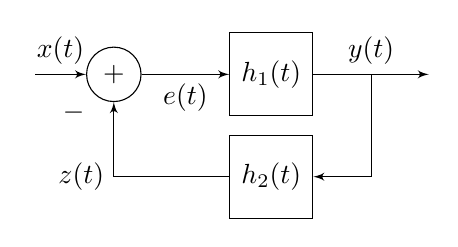
\begin{tikzpicture}[auto, node distance=2cm,>=latex']
    \node [input, name=rinput] (rinput) {};
    \node [sum, right of=rinput,label={below left:$-$}] (sum1) {+};
    \node [block, right of=sum1] (h1) {$h_1(t)$};
    \node [block, below of=h1,node distance=1.3cm] (h2) {$h_2(t)$};
    \node [output, right of=h1, node distance=2cm] (output) {};
    \draw [->] (rinput) -- node{$x(t)$} (sum1);
    \draw [->] (sum1) --node[name=z,anchor=north]{$e(t)$} (h1);
    \draw [->] (h1) -- node[name=y]{$y(t)$} (output);
    \draw [->] (y) |- (h2);
    \draw [->] (h2) -|node[name=x]{$z(t)$} (sum1);
\end{tikzpicture}
\caption{A simple feedback system}
\end{figure}
Here, 
\[y(t)=h_1(t)*e(t)\]
\[z(t)=y(t)*h_2(t)\]
\[e(t)=x(t)-z(t)\]
By transforming $y(t)=h_1(t)*e(t)$ and substituting $e$ and $z$,
\[Y(s)=H_1(s)(X(s)-Y(s)H_2(s))\]
Then we have
\[H(s)=\frac{Y(s)}{X(s)}=\frac{H_1(s)}{1+H_1(s)H_2(s)}\]

Read more in Ex. 9.28-9.31!
\section{$Z$-transform}
\underline{$z$-transform}
\begin{itemize}
    \item Generalization of DT-FT
    \item In LTI systems, when $x(n)=z^n$, $y(n)=H(z)z^n$, where $H(z)=\displaystyle{\sum_n{h(n)z^{-n}}}$
    \item If $z=e^{j2\pi f}$, then $H(z)$ becomes DT-FT.(i.e when $z$ is on the unit circle)
    \item In general, $z$ is an arbitrary complex value, so $z$-transform covers a wider range than DT-FT
    \[X(f)=\sum_n x(n)e^{-j2\pi fn}\]
    \[X(re^{j2\pi f})=\sum_n x(n)r^{-n}e^{-j2\pi fn}=\ft{x(n)r^{-n}}\]
    \item Convergence: $x(n)r^{-n}$ has a DT-FT.
    \item Ex. $x(n)=a^nu(n)$: right-sided signal
    \[X(z)=\frac{1}{1-az^{-1}}\:(\text{ROC: }|a|<|z|)\]
    out-sided in $z$-plane.
\end{itemize}
\underline{ROC in $z$-transform}
\begin{enumerate}
    \item ROC consists of ring(s) centered at the origin.
    \item No poles are included in the ROC
    \item $x(n)$: finite duration $\rightarrow$ ROC: entire $z$-plane except $z=0$ or $z=\infty$.
    \item $x(n)$ right-sided \& the circle $|z|=r_0$ is in the ROC $\rightarrow$ $|z| > r_0$ is in the ROC.
    \item $x(n)$ left-sided \& the circle $|z|=r_0$ is in the ROC $\rightarrow$ $0 < |z| < r_0$ is in the ROC.
    \item $x(n)$ two-sided \& $|z|=r_0$ is in the ROC $\rightarrow$ ROC is a ring including $|z|=r_0$.
    \item $X(z)$ rational, ROC is bounded by poles or extends to infinity
    \item $X(z)$ rational \& right-sided $\rightarrow$ ROC: outside outermost pole \& if causal, ROC includes $z=\infty$(i.e no $z^n(n>0)$ term).
    \item $X(z)$ rational \& left-sided $\rightarrow$ ROC: inside innermost pole \& if anticausal, ROC includes $z=0$(i.e no $z^{-n}(n>0)$ term).
\end{enumerate}
\underline{Inverse $z$-transform}
\begin{itemize}
    \item \[x(n)=\frac{1}{j2\pi}\oint_{|z|=r_0}X(z)z^{n-1}dz\]
    When $|z|=r_0$ is inside the ROC (as usual, integrated in the ccw direction).
    \item This can be derived from 
    \begin{align*}
        x(n)r_0^{-n}&=\int_1 X(r_0e^{j2\pi f})e^{j2\pi fn}df\:(\text{Inverse FT})\\
        x(n)&=\oint_{|z|=r_0} X(r_0e^{j2\pi f})(r_0e^{j2\pi f})^n \frac{dz}{zj2\pi}\:(\because\frac{dz}{df}=\frac{d(r_0e^{j2\pi f})}{df}=zj2\pi)\\
            &=\frac{1}{j2\pi}\oint_{|z|=r_0}X(z)z^{n-1}dz
    \end{align*}
    \item For rational $z$-transform, e.g for $\sum_{i=1}^{M}\frac{A_i}{1-az^{-1}}$, use partial fraction expansion. Note that $z^{-1}$ corresponds to time delay of 1, so use $z^{-1}$!
\end{itemize}
\underline{Geometric evaluation}
\begin{itemize}
    \item FT: use pole-zero plot and evaluate on the contour $|z|=1$
    \item Ex. $H(z)=\dfrac{1}{1-az^{-1}}$: pole at $a$. zero at $0$. ROC $|z|>|a|$ must contain $|z|=1$, so $|a|<1$.
    \item $|H(f)|$ is $|z-0|$(product of distances between $z$ and the zeros) over $|z-a|$(product of distances between $z$ and the poles) when $z=e^{j2\pi f}$, $\angle H(f)$ is $\angle(e^{j2\pi f}-0)$(sum of angles of $z-$(zeros)) minus $\angle(e^{j2\pi f}-a)$(sum of angles of $z-$(poles)).
\end{itemize}
\underline{Properties of ROC}
\begin{itemize}
\item Linearity: ROC: $R_1\bigcap R_2$
\item Time shifting: $x(n-n_0)\leftrightarrow z^{-n_0}X(z)$, ROC: $R$ except addition or deletion at $\infty$. $0$ due to the $z^n$ term.
\item Scaling in $z$(shift in $f$): $z_0^nx(n)\leftrightarrow X\left(\dfrac{z}{z_0}\right)$, ROC: $|z_0|R$
\item Time reversal: $x(-n)\leftrightarrow X(z^{-1})$, ROC: $\dfrac{1}{R}$
\item Time expansion: $x_{(k)}(n)\leftrightarrow X(z^k)$, ROC: $R^{1/k}$
\item Conjugate: $x^*(n)\leftrightarrow X^*(z^*)$, ROC: same.
\item Convolution: $x_1(n)*x_2(n)\leftrightarrow X_1(z)X_2(z)$, ROC: $R_1\bigcap R_2\subseteq R$
\item Differentiation in $z$: $nx(n)\leftrightarrow -z\dfrac{dX(z)}{dz}$, ROC: same.
\item Initial value theorem: If $x(n)=0$ for $n<0$,
\[x(0)=\lim_{z\rightarrow\infty}X(z)\]
\end{itemize}
\underline{LTI system \& $z$-transform}
\begin{itemize}
    \item In DT LTI, $Y(z)=H(z)X(z)$, when $H(z)$ is the system function or the transfer function, becomes the ''frequency response" if evaluated for $z=e^{j2\pi f}$
    \item Causality: $h(n)=0$ for $n < 0$: right-sided impulse response function: ROC is out-sided, i.e it is the exterior of a circle including infinity. If the system function is rational, the system is causal iff (a) the ROC is outside the outermost pole and (b) $\deg{N(z)} \le \deg{D(z)}$ ($N$: numerator, $D$: denominator), so the ROC contains $\infty$(no $z^n(n>0)$ term).
    \item Stability: An LTI system is stable iff the ROC of $H(z)$ includes $|z|=1$. A causal LTI system with a rational system function is stable iff all poles of $H(z)$ lies inside the unit circle.
    \item Ex. 10.25 LCCDE(Linear Constant Coefficient Difference Equation)
    \[y(n)-\frac{1}{2}y(n-1)=x(n)+\frac{1}{3}x(n-1)\]
    The system function becomes
    \[H(z)=\frac{1+z^{-1}/3}{1-z^{-1}/2}=\frac{z+1/3}{z-1/2}\]
    The pole $1/2$ is inside the unit circle. Assuming that this system is causal, we can assure that the ROC is $|z|>\dfrac{1}{2}$. Then the system is also stable. Solve also examples 10.26, 10.27!
\end{itemize}
\underline{System function algebra and block diagrams}
\begin{figure}[htb]
\centering
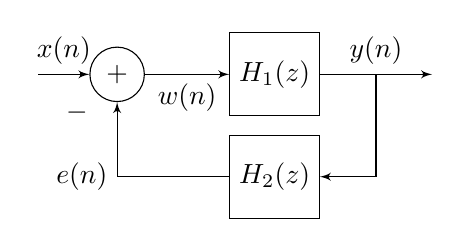
\begin{tikzpicture}[auto, node distance=2cm,>=latex']
    \node [input, name=rinput] (rinput) {};
    \node [sum, right of=rinput,label={below left:$-$}] (sum1) {+};
    \node [block, right of=sum1] (h1) {$H_1(z)$};
    \node [block, below of=h1,node distance=1.3cm] (h2) {$H_2(z)$};
    \node [output, right of=h1, node distance=2cm] (output) {};
    \draw [->] (rinput) -- node{$x(n)$} (sum1);
    \draw [->] (sum1) --node[name=z,anchor=north]{$w(n)$} (h1);
    \draw [->] (h1) -- node[name=y]{$y(n)$} (output);
    \draw [->] (y) |- (h2);
    \draw [->] (h2) -|node[name=x]{$e(n)$} (sum1);
\end{tikzpicture}
\caption{A simple feedback system, DT}
\end{figure}

We have \[\frac{Y(z)}{X(z)}=H(z)=\frac{H_1(z)}{1+H_1(z)H_2(z)}\]
\begin{itemize}
    \item Ex1: $H(z)=\dfrac{1}{1-\dfrac{1}{4}z^{-1}}$. $y(n)-\dfrac{1}{4}y(n-1)=x(n)$ can be obtained by the feedback system above when $H_1(z)=1$ is the identity system and $H_2(z)=-\dfrac{1}{4}z^{-1}$: $H_2(z)$ can be obtained by changing the - sign next to $\bigoplus$ to +, and cascading $1/4$(constant multiplication) with $z^{-1}$(time delay).
    \item Ex2: $H(z)=\dfrac{1-2z^{-1}}{1-\dfrac{1}{4}z^{-1}}$. $y(n)-\dfrac{1}{4}y(n-1)=x(n)-2x(n-1)$ can be obtained by cascading the system in Ex2 with the system $1-2z^{-1}$.
\end{itemize}
\begin{figure}[htb]
\centering
\begin{tikzpicture}[auto, node distance=2cm,>=latex']
    \node [input, name=rinput] (rinput) {};
    \node [sum, right of=rinput,label={below left:$+$}] (sum1) {+};
    \node [block, below right of=sum1, node distance=3cm](c1){$\dfrac{1}{4}$};
    \node [output, right of=sum1, node distance=4cm] (output1) {};
    \node [block, below of=output1, node distance=1.1cm] (z1) {$z^{-1}$};
    \node [output, right of=output1] (out){};
    \node [block, below of=out, node distance=1.1cm] (z2) {$z^{-1}$};
    \node [sum, right of=out, label={below left:$+$}, node distance=4cm] (sum2) {+};
    \node [block, below left of=sum2, node distance=3cm](c2){$-2$};
    \node [output, right of=sum2, node distance=1.3cm] (output2){};
    \draw [->] (rinput) -- node{$x(n)$} (sum1);
    \draw [-] (sum1) --node[name=z, anchor=north]{} (output1);
    \draw [->] (output1) -- node[name=y]{} (z1);
    \draw [->] (z1) |- (c1);
    \draw [->] (c1) -|node[name=x]{} (sum1);
    \draw [-] (output1) |- (out);
    \draw [->] (out) -- (sum2);
    \draw [->] (out) -- (z2);
    \draw [->] (z2) |- (c2);
    \draw [->] (c2) -| (sum2);
    \draw [->] (sum2) --node[name=y]{$y(n)$} (output2);
\end{tikzpicture}
\caption{An implementation of Ex2}
\end{figure}
\begin{itemize}
    \item Ex3. $H(z)=\dfrac{1}{(1+\dfrac{1}{2}z^{-1})(1-\dfrac{1}{4}z^{-1})}$, $y(n)+\dfrac{1}{4}y(n-1)-\dfrac{1}{8}y(n-2)=x(n)$: This can be rearranged to $y(n)=x(n)-\dfrac{1}{4}y(n-1)+\dfrac{1}{8}y(n-2)$, which is a feedback system obtained by adding $x(n)$ to two delayed versions of $y(n)$: $y(n-1)$ by passing through one delay, which is delayed again to become $y(n-2)$, the second version. (Direct)
    \item (Cascaded) Or this can be obtained from cascading, like Figure 2.
    \item (Parallel) Or this can be obtained by expanding in partial fractions
    \[H(z)=\dfrac{\dfrac{2}{3}}{1+\dfrac{1}{2}z^{-1}}+\dfrac{\dfrac{1}{3}}{1-\dfrac{1}{4}z^{-1}}\] and adding the outputs of each system(each partial fraction).
    \item Each circuit implementation has differences in cost and speed.
\end{itemize}
\begin{figure}[htb]
\centering
\begin{tikzpicture}[auto, node distance=2cm,>=latex']
    \node [input, name=rinput] (rinput) {};
    \node [sum, right of=rinput,label={below left:$+$}] (sum1) {+};
    \node [block, below right of=sum1, node distance=3cm](c1){$-\dfrac{1}{4}$};
    \node [output, right of=sum1, node distance=4cm] (output1) {};
    \node [block, below of=output1, node distance=1.1cm] (z1) {$z^{-1}$};
    \node [output, right of=output1] (out){};
    \node [block, below of=z1, node distance=2cm] (z2) {$z^{-1}$};
    \node [sum, below of=sum1, label={below left:$+$}, node distance=2.1cm] (sum2) {+};
    \node [block, below right of=sum2, node distance=3cm](c2){$\dfrac{1}{8}$};
    \draw [->] (rinput) -- node{$x(n)$} (sum1);
    \draw [-] (sum1) --node[name=z, anchor=north]{} (output1);
    \draw [->] (output1) -- node[name=y]{} (z1);
    \draw [->] (z1) |- (c1);
    \draw [->] (c1) -- (sum2);
    \draw [->] (output1) --node[name=y]{$y(n)$} (out);
    \draw [->] (z1) -- (z2);
    \draw [->] (z2) |- (c2);
    \draw [->] (c2) -| (sum2);
    \draw [->] (sum2) -- (sum1);
\end{tikzpicture}
\caption{Direct implementation of Ex3}
\end{figure}
\end{document}